% Options for packages loaded elsewhere
\PassOptionsToPackage{unicode}{hyperref}
\PassOptionsToPackage{hyphens}{url}
\PassOptionsToPackage{dvipsnames,svgnames,x11names}{xcolor}
%
\documentclass[
]{scrbook}
\usepackage{amsmath,amssymb}
\usepackage{lmodern}
\usepackage{iftex}
\ifPDFTeX
  \usepackage[T1]{fontenc}
  \usepackage[utf8]{inputenc}
  \usepackage{textcomp} % provide euro and other symbols
\else % if luatex or xetex
  \usepackage{unicode-math}
  \defaultfontfeatures{Scale=MatchLowercase}
  \defaultfontfeatures[\rmfamily]{Ligatures=TeX,Scale=1}
\fi
% Use upquote if available, for straight quotes in verbatim environments
\IfFileExists{upquote.sty}{\usepackage{upquote}}{}
\IfFileExists{microtype.sty}{% use microtype if available
  \usepackage[]{microtype}
  \UseMicrotypeSet[protrusion]{basicmath} % disable protrusion for tt fonts
}{}
\makeatletter
\@ifundefined{KOMAClassName}{% if non-KOMA class
  \IfFileExists{parskip.sty}{%
    \usepackage{parskip}
  }{% else
    \setlength{\parindent}{0pt}
    \setlength{\parskip}{6pt plus 2pt minus 1pt}}
}{% if KOMA class
  \KOMAoptions{parskip=half}}
\makeatother
\usepackage{xcolor}
\IfFileExists{xurl.sty}{\usepackage{xurl}}{} % add URL line breaks if available
\IfFileExists{bookmark.sty}{\usepackage{bookmark}}{\usepackage{hyperref}}
\hypersetup{
  pdftitle={Statistical Techniques for Biological and Environmental Sciences},
  pdfauthor={Brad Duthie},
  colorlinks=true,
  linkcolor={blue},
  filecolor={Maroon},
  citecolor={Blue},
  urlcolor={Blue},
  pdfcreator={LaTeX via pandoc}}
\urlstyle{same} % disable monospaced font for URLs
\usepackage{longtable,booktabs,array}
\usepackage{calc} % for calculating minipage widths
% Correct order of tables after \paragraph or \subparagraph
\usepackage{etoolbox}
\makeatletter
\patchcmd\longtable{\par}{\if@noskipsec\mbox{}\fi\par}{}{}
\makeatother
% Allow footnotes in longtable head/foot
\IfFileExists{footnotehyper.sty}{\usepackage{footnotehyper}}{\usepackage{footnote}}
\makesavenoteenv{longtable}
\usepackage{graphicx}
\makeatletter
\def\maxwidth{\ifdim\Gin@nat@width>\linewidth\linewidth\else\Gin@nat@width\fi}
\def\maxheight{\ifdim\Gin@nat@height>\textheight\textheight\else\Gin@nat@height\fi}
\makeatother
% Scale images if necessary, so that they will not overflow the page
% margins by default, and it is still possible to overwrite the defaults
% using explicit options in \includegraphics[width, height, ...]{}
\setkeys{Gin}{width=\maxwidth,height=\maxheight,keepaspectratio}
% Set default figure placement to htbp
\makeatletter
\def\fps@figure{htbp}
\makeatother
\setlength{\emergencystretch}{3em} % prevent overfull lines
\providecommand{\tightlist}{%
  \setlength{\itemsep}{0pt}\setlength{\parskip}{0pt}}
\setcounter{secnumdepth}{5}
\usepackage{booktabs}
\usepackage{amsthm}
\makeatletter
\def\thm@space@setup{%
  \thm@preskip=8pt plus 2pt minus 4pt
  \thm@postskip=\thm@preskip
}
\makeatother
\ifLuaTeX
  \usepackage{selnolig}  % disable illegal ligatures
\fi
\usepackage[]{natbib}
\bibliographystyle{apalike}

\title{Statistical Techniques for Biological and Environmental Sciences}
\author{Brad Duthie}
\date{2022-10-23}

\begin{document}
\maketitle

{
\hypersetup{linkcolor=}
\setcounter{tocdepth}{1}
\tableofcontents
}
\hypertarget{preface}{%
\chapter*{Preface}\label{preface}}
\addcontentsline{toc}{chapter}{Preface}

Welcome to the module. This workbook will be used throughout the semester and contain all of the information that you need for the statistical techniques (SCIU4T4) module.

\hypertarget{what-is-statistics}{%
\section{What is statistics?}\label{what-is-statistics}}

An explanation of the material, and what will be taught.

\hypertarget{why-this-module-is-important}{%
\section{Why this module is important}\label{why-this-module-is-important}}

Some discussion of module importance

\hypertarget{teaching-overview}{%
\section{Teaching overview}\label{teaching-overview}}

Here is how you will be taught, with online lectures, reading assignments, and face-to-face practicals.

\hypertarget{assessment-overview}{%
\section{Assessment overview}\label{assessment-overview}}

You will have one formative test and two summatitive tests. You will also have one mock exam and one exam exam.

\hypertarget{test-1f}{%
\subsection{Test 1F}\label{test-1f}}

Information about Test 1F

\hypertarget{test-1s}{%
\subsection{Test 1S}\label{test-1s}}

Information about Test 1S

\hypertarget{test-2s}{%
\subsection{Test 2S}\label{test-2s}}

Information about Test 1S

\hypertarget{mock-exam}{%
\subsection{Mock Exam}\label{mock-exam}}

Information about the mock exam

\hypertarget{exam}{%
\subsection{Exam}\label{exam}}

Information about the exam

\hypertarget{intro_jamovi}{%
\section{Jamovi statistical software}\label{intro_jamovi}}

Introduction to \href{https://www.jamovi.org/}{Jamovi}, and why we are using it instead of other software.

\hypertarget{textbooks}{%
\section{Textbooks}\label{textbooks}}

Introduction to the primary textbook \href{https://www.learnstatswithjamovi.com/}{Learning statistics with jamovi}, and a mention of other sources.

\hypertarget{canvas}{%
\section{Canvas}\label{canvas}}

How we will use Canvas, and how this book relates to it (Learning and Teaching content, where lectures, assessments, and discussions can be found).

\hypertarget{timetable}{%
\section{Timetable}\label{timetable}}

\hypertarget{part-background-mathematics-and-data-organisation}{%
\part{Background mathematics and data organisation}\label{part-background-mathematics-and-data-organisation}}

\hypertarget{week-1-overview}{%
\chapter*{Week 1 Overview}\label{week-1-overview}}
\addcontentsline{toc}{chapter}{Week 1 Overview}

In week 1, we will focus on a refresher of some necessary background mathematics for this module. We will then turn to the topic of how to organise data sets. We will then practice organising datasets and saving them in a usable format.

Week: 1
Dates:
Suggested Readings: Textbook intro, Hadley's paper
Assessments: Practice quiz
Practical: Quick summary of topics covered

\hypertarget{background_mathematics}{%
\chapter{Background mathematics}\label{background_mathematics}}

Some of this will be review, but it is important. Suggested reading for this (some mathematics text).

\hypertarget{numbers-and-operations}{%
\section{Numbers and operations}\label{numbers-and-operations}}

A very broad reminder of mathematics, which you will need for this module

\hypertarget{order-of-operations}{%
\section{Order of operations}\label{order-of-operations}}

This is easy to forget

\hypertarget{data_organisation}{%
\chapter{Data organisation}\label{data_organisation}}

It is important to organise data properly so that statistical analysis can be done. Here I explain the tidy approach to data. Suggested reading Hadley Wickam's paper.

\hypertarget{tidy-data}{%
\section{Tidy data}\label{tidy-data}}

\hypertarget{data-files}{%
\section{Data files}\label{data-files}}

\hypertarget{practical-preparing-real-datasets}{%
\chapter{\texorpdfstring{\emph{Practical}: Preparing real datasets}{Practical: Preparing real datasets}}\label{practical-preparing-real-datasets}}

In this practical, we will use a spreadsheet to organise datastes.

\hypertarget{libreoffice-calc}{%
\section{LibreOffice Calc}\label{libreoffice-calc}}

LibreOffice Calc is a free and open source spreadsheet program. The instructions for this section will be identical to the more popular commercial Microsoft Excel.

\hypertarget{exercise-organising-data-1}{%
\section{Exercise Organising data 1}\label{exercise-organising-data-1}}

Walks through Exercise 1.3.2

\hypertarget{exercise-organising-data-2}{%
\section{Exercise Organising data 2}\label{exercise-organising-data-2}}

Walks through Exercise 1.3.3

\hypertarget{exercise-organising-data-3}{%
\section{Exercise Organising data 3}\label{exercise-organising-data-3}}

Walks through Exercise 1.3.4, saving all of these as CSV files

\hypertarget{summary-of-exercises-and-why-they-are-useful.}{%
\section{Summary of exercises and why they are useful.}\label{summary-of-exercises-and-why-they-are-useful.}}

\hypertarget{part-statistical-concepts}{%
\part{Statistical concepts}\label{part-statistical-concepts}}

\hypertarget{week-2-overview}{%
\chapter*{Week 2 Overview}\label{week-2-overview}}
\addcontentsline{toc}{chapter}{Week 2 Overview}

\begin{longtable}[]{@{}
  >{\raggedright\arraybackslash}p{(\columnwidth - 2\tabcolsep) * \real{0.3269}}
  >{\raggedright\arraybackslash}p{(\columnwidth - 2\tabcolsep) * \real{0.6731}}@{}}
\toprule
\endhead
\textbf{Dates} & 30 January 2023 - 3 February 2023 \\
\textbf{Reading} & \textbf{Required:} SCIU4T4 Workbook chapters 4-8 \\
& \textbf{Recommended:} \citet{Navarro2022} \href{https://davidfoxcroft.github.io/lsj-book/getting-started-with-jamovi.html\#the-spreadsheet}{Section 3.3}-\href{https://davidfoxcroft.github.io/lsj-book/getting-started-with-jamovi.html\#summary-1}{3.9} \\
& \textbf{Optional:} \citet{Rowntree2018} Chapter 2 \\
& \textbf{Advanced:} \citet{Spiegelhalter2019} Chapters 1-3 \\
\textbf{Lectures} & 2.0: Introduction to Week 1 (2 min.) \\
& 2.1: Why study statistics? (18 min.) \\
& 2.2: Populations and samples (7 min.) \\
& 2.3: Types of variables (11 min.) \\
& 2.4: Units, precision, and accuracy (9 min.) \\
& 2.5. Uncertainty propagation (11 min.) \\
\textbf{Practical} & Introduction to Jamovi \\
\textbf{Assessments} & Week 2 Practice quiz on Canvas \\
\bottomrule
\end{longtable}

In \protect\hyperlink{Chapter_4}{Chapter 4}, we focus on key concepts that will be used throughout this module.
In particular, it is important to understand the difference between a \textbf{population} and a \textbf{sample}, and to recognise that there are many types of variables in statistics.

In \protect\hyperlink{Chapter_5}{Chapter 5}, we look at different variable types. Different types of variables have different characteristics, which will affect how these variables are best visualised in figures and analysed with statistical hypothesis tests introduced later in the semester.
Identifying variable types will therefore be important, both for module assessments and when working with new datasets.
A variable's type will rarely be stated explicitly when doing scientific research, and will not always be provided in assessments for this module.
Being able to infer variable type is therefore an important skill.

\protect\hyperlink{Chapter_6}{Chapter 6} focus on units of measurement, and how these units are communicated in text.
Units are essential in scientific measurement, and we will use them throughout the module to indicate the type and scale of data measurement.
We are not expecting you to memorise all scientific units, so a \protect\hyperlink{appendixA_units}{table on units} is provided at the end of this workbook.

\protect\hyperlink{Chapter_7}{Chapter 7} will introduce the propogation of measurement errors.
This is important to understand because no measurement is perfectly accurate, and predicting how errors in measurement combine is fundamental to understanding measurement accuracy.

Finally, \protect\hyperlink{Chapter_8}{Chapter 8} guides you through the Week 2 practical, which is an introduction to Jamovi.
This aim of this practical is to become familiar with the Jamovi interface and comfortable importing data into Jamovi to collect some descriptive statistics.

\hypertarget{Chapter_4}{%
\chapter{Populations and samples}\label{Chapter_4}}

When we collect data, we are recording some kind of observation or measurement.
If we are working in a forest, for example, we might want to measure the heights of different trees, or measure the concentration of carbon in the soil.
The idea might be to use these measurements to make some kind of inference about the forest.
But as scientists, we are almost always limited in the amount of data that we can collect.
We cannot measure everything, so we need to collect a \emph{sample} of data and use it to make inferences about the \emph{population} of interest.
For example, while we probably cannot measure the height of every tree in a forest, nor can we measure the concentration of carbon at every possible location in the forest's soil, we can collect a smaller number of measurements and still make useful conclusions about overall forest trees and carbon concentration.

Statistics thereby allows us to approximate properties of entire populations from a limited number of samples.
This needs to be done with caution, but before getting into the details of how, it is important to understand the difference between a \textbf{population} and a \textbf{sample} to avoid confusing these two concepts.
A \textbf{population} is the entire set of possible observations that could be collected.
Some examples will make it easier to understand:

\begin{itemize}
\tightlist
\item
  All of the genes in the human genome
\item
  All individuals of voting age in Scotland
\item
  All common pipistrelle bats in the United Kingdom
\end{itemize}

These populations might be important for a particular research question.
For example, we might want to know something about the feeding behaviours of pipistrelle bats in the UK.
But there is no way that we can find and observe the behaviour of every bat, so we need to take a subset of the population (a sample) instead.
Examples of samples include the following:

\begin{itemize}
\tightlist
\item
  A selection of 20 human genes
\item
  A pub full of Scottish voters
\item
  40 caught common pipistrelle bats
\end{itemize}

It is important to recognise that the word ``population'' means something slightly different in statistics than it does in biology.
A biological population, for example, could be defined as all of the individuals of the same species in the same general location.
A statistical population, in contrast, refers to a set of observations (i.e., things that we can measure).
\citet{Sokal1995} provide a more technical definition for ``population'',

\begin{quote}
In statistics, population always means the \emph{totality of individual observations about which inferences are to be made, existing anywhere in the world or at least within a definitely specified sampling area limited in space and time} {[}p.~9, emphasis theirs{]}.
\end{quote}

They define a sample to be ``a collection of individual observations selected by a specified procedure'' \citep{Sokal1995}.
For our purposes, it is not necessary to be able to recite the technical definitions, but it is important to understand the relationship between a population and a sample.
When we collect data, we are almost always taking a small sample of observations from a much larger number of possible observations in a population.

\begin{figure}
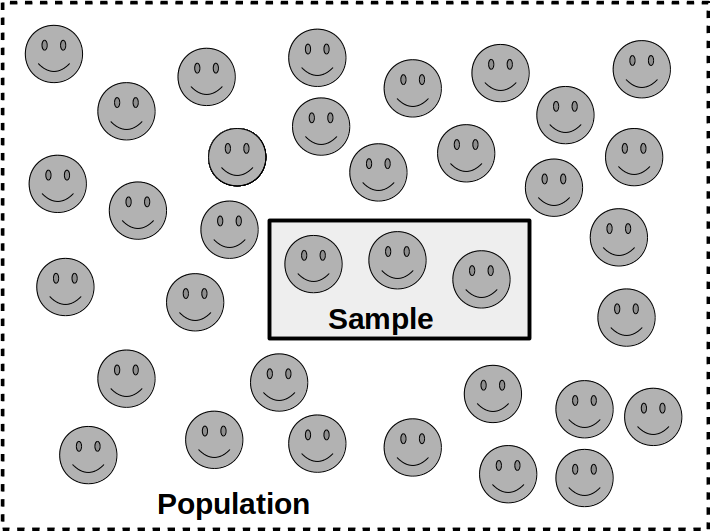
\includegraphics[width=1\linewidth]{img/population_vs_sample} \caption{A conceptual figure illustrating how a statistical population relates to a statistical sample. The population is represented by 35 smiling faces enclosed within a dashed box. The sample is represented by a solid box within the dashed box, within which there are 3 smiling faces. Hence, we have a sample of 3 measurements from the total population.}\label{fig:unnamed-chunk-1}
\end{figure}

\hypertarget{Chapter_5}{%
\chapter{Types of variables}\label{Chapter_5}}

A variable is any property that is measured in an observation \citep{Sokal1995}; i.e., anything that varies among things that we can measure \citep{Dytham2011}.
We can summarise how these measurements vary with summary statistics, or visually with figures.
Often, we will want to predict one variable from a second variable.
In this case, the variable that we want to predict is called the \textbf{response variable}, also known as the \textbf{dependent variable} or \textbf{Y} variable (`dependent' because it \emph{depends} on other variables, and `Y' because this is the letter we often use to represent it).
The variable that we use to predict our response variable is the \textbf{explanatory variable}, also known as the \textbf{independent variable} or \textbf{X} variable (`independent' because it does not depend on other variables, and `X' because this is the letter most often used to represent it).
There are several different types of variables:

\begin{itemize}
\item
  \textbf{Categorical} variables take on a fixed number of discrete values \citep{Spiegelhalter2019}.
  In other words, the measurement that we record will assign our data to a specific category.
  Examples of categorical variables include species (e.g., ``Robin'', ``Nightingale'', ``Wren'') or life history stage (e.g., ``egg'', ``juvenile'', ``adult'').
  Categorical variables can be either nominal or ordinal.

  \begin{itemize}
  \tightlist
  \item
    \textbf{Nominal} variables do not have any inherent order (e.g., classifying land as ``forest'', ``grassland'', or ``urban'').
  \item
    \textbf{Ordinal} variables do have an inherent order (e.g., ``low'', ``medium'', and ``high'' elevation).
  \end{itemize}
\item
  \textbf{Quantitative} variables are variables represented by numbers that reflect a magnitude.
  That is, unlike categorical variables, we are collecting numbers that really mean something tangible (in contrast, while we might represent low, medium, and high elevations with the numbers 1, 2, and 3, respectively, this is just for convenience; a value of `2' does not always mean `medium').
  Categorical variables can be either discrete or continuous.

  \begin{itemize}
  \item
    \textbf{Discrete} variables can take only certain values.
    For example, if we want to record the number of species in a forest, then our variable can only take discrete counts (i.e., integer values).
    There could conceivably be any whole number of species (1, 2, 3, etc.), but there could not be 2.51 different species in a forest; that does not make sense.
  \item
    \textbf{Continuous} variables can take any real value within some range of values (i.e., any number that can be represented by a decimal).
    For example, we could measure height to as many decimals as our measuring device will allow, with a range of values from zero to the maximum possible height of whatever it is we are measuring.
    Similarly, we could measure temperature to any number of decimals, at least in theory, so temperature is a continuous variable.
  \end{itemize}
\end{itemize}

The reason for organising variables into all of these different types is that different types of variables need to be handled in different ways.
For example, it would not make sense to visualise a nominal variable in the same way as a continuous variable.
Similarly, the choice of statistical test to apply to answer a statistical question will almost always depend on the types of variables involved.
If presented with a new data set, it is therefore very important to be able to interpret the different variables and apply the correct statistical techniques (this will be part of the assessment for this module).

\hypertarget{Chapter_6}{%
\chapter{Accuracy, precision, and units}\label{Chapter_6}}

The science of measurements is called ``metrology'', which, among other topics, focuses on measurement accuracy, precision, and units \citep{Rabinovich2013}.
We will not discuss these topics in depth, but they are important for statistical techniques because measurement, in the broadest sense of the word, is the foundation of data collection.
When collecting data, we want measurements to be accurate, precise, and clearly defined.

\hypertarget{accuracy}{%
\section{Accuracy}\label{accuracy}}

When we collect data, we are trying to obtain information about the world.
We might, for example, want to know the number of seedlings in an area of forest, them temperature of the soil at a location, or the mass of a particular animal in the field.
To get this information, we need to make measurements.
Some measurements can be collected by simple observation (e.g., counting seedlings), while others will require measuring devices such as a thermometer (for measuring temperature) or scale (for measuring mass).
All of these measurements are subject to error.
The \emph{true} value of whatever it is that we are trying to measure (called the ``measurand'') can differ from what we record when collecting data.
This is true even for simple observations (e.g., we might miscount seedlings), so it is important to recognise that the data we collect comes with some uncertainty.
The \textbf{accuracy} of a measurement is defined by how close the measurement is to the \emph{true} value of what we are trying to measure \citep{Rabinovich2013}.

\hypertarget{precision}{%
\section{Precision}\label{precision}}

The \textbf{precision} of a measurement is how consistent it will be if measurement is replicated multiple times.
In other words, precision describes how similar measurements are expected to be.
If, for example, a scale measures an object to be the exact same mass ever time it is weighed (regardless of whether the mass is accurate), then the measurement is highly precise.
If, however, the scale measures a different mass each time the object is weighed (for this hypothetical, assume that the true mass of the object does not change), then the measurement is not as precise.

One way to visualise the difference between accuracy and precision is to imagine a set of targets, with the centre of the target representing the true value of what we are trying to measure (Figure 6.1)\footnote{This figure was released into the public domain by \href{https://commons.wikimedia.org/wiki/File:Accuracy-vs-precision-nl.svg}{Egon Willighagen} on 8 March 2014.}.

\begin{figure}
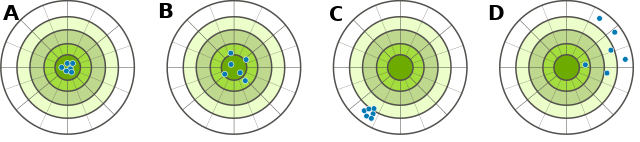
\includegraphics[width=1\linewidth]{img/accuracy_vs_precision} \caption{A conceptual figure illustrating the difference between accuracy and precision. Points in (A) are both accurate and precise, points in (B) are accurate, but not precise, points in (C) are precise but not accurate, and points in (D) are neither accurate nor precise.}\label{fig:unnamed-chunk-2}
\end{figure}

Note again that accuracy and precision are not necessarily the same.
Measurement can be accurate but not precise (Figure 6.1B) or precise but not accurate (Figure 6.1C).

\hypertarget{systems-of-units}{%
\section{Systems of units}\label{systems-of-units}}

Scientific units are standardised with the Système International D'Unités (SI).
Having standardised units of measurement is highly important to ensure measurement accuracy \citep{Quinn1995}.
Originally, these units were often defined in terms of physical artefacts.
For example, the kilogram (kg) was once defined by physical cylinder metal housed in the Buereau International des Poids et Mesures (BIPM).
In other words, the mass of a metal sitting at the BIPM \emph{defined} what a kg was, with the mass of every other measurement being based on this physical object \citep{Quinn1995}.
This can potentially present a problem if the mass of that one object changes over time, thereby causing a change in how a kg is defined.
Where possible, it is therefore preferable to define units in terms of fundamental constants of nature.
In 2019, for example, the kg was redefined in terms of the Planck constant, a specific atomic transition frequency, and the speed of light \citep{Stock2019}.
This ensures that measurements of mass remain accurate over time because what a kg represents in terms of mass cannot change.

We can separate units into base units and derived units.
Table 6.1 below lists some common base units for convenience \citep{Quinn1995}.
You do not need to memorise these units, but it is good to be familiar with them.
We will use these units throughout the module.

\begin{longtable}[]{@{}lll@{}}
\caption{Base units of SI measurements. For details see \citet{Quinn1995}.}\tabularnewline
\toprule
\textbf{Measured Quantity} & \textbf{Name of SI unit} & Symbol \\
\midrule
\endfirsthead
\toprule
\textbf{Measured Quantity} & \textbf{Name of SI unit} & Symbol \\
\midrule
\endhead
Mass & kilogram & \(kg\) \\
Length & metre & \(m\) \\
Time & second & \(s\) \\
Electric current & ampere & \(A\) \\
Temperature & kelvin & \(K\) \\
Amount of a substance & mole & \(mol\) \\
Luminous intensity & candela & \(cd\) \\
\bottomrule
\end{longtable}

We can also define derived SI units from the base units of Table 6.1; examples of these derived SI units are provided in Table 6.2 below.
Again, you do not need to memorise these units, but it is good to be aware of them.

\begin{longtable}[]{@{}
  >{\raggedright\arraybackslash}p{(\columnwidth - 8\tabcolsep) * \real{0.2000}}
  >{\raggedright\arraybackslash}p{(\columnwidth - 8\tabcolsep) * \real{0.1565}}
  >{\raggedright\arraybackslash}p{(\columnwidth - 8\tabcolsep) * \real{0.1043}}
  >{\raggedright\arraybackslash}p{(\columnwidth - 8\tabcolsep) * \real{0.2435}}
  >{\raggedright\arraybackslash}p{(\columnwidth - 8\tabcolsep) * \real{0.2957}}@{}}
\caption{Examples of derived SI units.}\tabularnewline
\toprule
\begin{minipage}[b]{\linewidth}\raggedright
\textbf{Measured Quantity}
\end{minipage} & \begin{minipage}[b]{\linewidth}\raggedright
\textbf{Name of unit}
\end{minipage} & \begin{minipage}[b]{\linewidth}\raggedright
\textbf{Symbol}
\end{minipage} & \begin{minipage}[b]{\linewidth}\raggedright
\textbf{Definition in SI units}
\end{minipage} & \begin{minipage}[b]{\linewidth}\raggedright
\textbf{Alternative in derived units}
\end{minipage} \\
\midrule
\endfirsthead
\toprule
\begin{minipage}[b]{\linewidth}\raggedright
\textbf{Measured Quantity}
\end{minipage} & \begin{minipage}[b]{\linewidth}\raggedright
\textbf{Name of unit}
\end{minipage} & \begin{minipage}[b]{\linewidth}\raggedright
\textbf{Symbol}
\end{minipage} & \begin{minipage}[b]{\linewidth}\raggedright
\textbf{Definition in SI units}
\end{minipage} & \begin{minipage}[b]{\linewidth}\raggedright
\textbf{Alternative in derived units}
\end{minipage} \\
\midrule
\endhead
Energy & Joule & \(J\) & \(m^{2}\) \(kg\) \(s^{-2}\) & \(N\) \(m\) \\
Force & Newton & \(N\) & \(m\) \(kg\) \(s^{-2}\) & \(J\) \(m^{-1}\) \\
Pressure & Pascal & \(Pa\) & \(kg\) \(m^{-1}\) \(s^{-2}\) & \(N\) \(m^{-2}\) \\
Power & Watt & \(W\) & \(m^{-2}\) \(kg\) \(s^{-3}\) & \(J\) \(s^{-1}\) \\
Frequency & Hertz & \(Hz\) & \(s^{-1}\) & \\
Radioactivity & Becquerel & \(Bq\) & \(s^{-1}\) & \\
\bottomrule
\end{longtable}

When numbers are associated with units, it is important to recognise that the units must be carried through and combined when calculating equation.
As a very simple example, if want to know the speed at which an object is moving, and we find that it has moved 10 metres in 20 seconds, then we calculate the speed and report the correct units as below,

\[speed = \frac{10\:m}{20\:s} = 0.5\:m/s = 0.5\:m\:s^{-1}.\]
Notice that the final units are in metres per second, which can be written as \(m/s\) or \(m\:s^{-1}\) (remember that raising \(s\) to the \(-1\) power is the same as \(1/s\); see below for a quick reminder about superscripts).
It is a common error to calculate just the numeric components of a calculation and ignore the associated units.
Often on assessments, we will ask you not to include units in your answer (this is just for convenience on the tests and exam), but recognising that units are also part of calculations is important.

\hypertarget{other-examples-of-units}{%
\section{Other examples of units}\label{other-examples-of-units}}

Remember that an exponent (indicated by a superscript, e.g., the 3 in \(m^{3}\)) indicates the number of times to multiply a base by itself, so \(m^{3} = m \times m \times m\).

\hypertarget{units-of-density}{%
\subsection{Units of density}\label{units-of-density}}

Density (\(\rho\)) is calculated by,

\[\rho = \frac{mass}{volume} = \frac{kg}{m^{3}}.\]

The units of density are therefore mass per unit volume, \(kg\:m^{-3}\).

\hypertarget{mass-of-metal-discharged-from-a-catchment}{%
\subsection{Mass of metal discharged from a catchment}\label{mass-of-metal-discharged-from-a-catchment}}

The mass of metal carried by a stream per unit time (\(M\)) is given by multiplying the concentration of metal per unit volume (\(C\)) of water by the volume of water discharged per unit time (\(V\)),

\[M = C \times V.\]
This equation is useful in showing how units can cancel each other out.
If we calculate the above with just the units (ignoring numbers for \(C\) and \(V\)),

\[M = \frac{mg}{l} \times \frac{l}{s} = \frac{mg}{s}.\]

Notice above how the \(l\) units on the top and bottom of the equation cancel each other out, so we are left with just \(mg/s\).

\hypertarget{soil-carbon-inventories}{%
\subsection{Soil carbon inventories}\label{soil-carbon-inventories}}

For one final example, the inventory of carbon \(I\) within a soil is given by the specific carbon concentration \(C\) (\(g\) of carbon per \(kg\) of soil), multiplied by the depth of soil analysed (\(D\), \(m\)), and by the density (\(\rho\), \(kg\:m^{-3}\)),

\[I = C \times D \times \rho = \frac{g\times m \times kg}{kg \times m^{3}} = \frac{g}{m^{2}} = g\:m^{-2}.\]
Notice above how the \(kg\) on the top and bottom of the fraction cancel each other out, and how one \(m\) on the top cancels out one \(m\) on the bottom, so that what we are left with is grams per metre squared (\(g\:m^{-2}\)).

\hypertarget{Chapter_7}{%
\chapter{Uncertainty propogation}\label{Chapter_7}}

Nothing can be measured with perfect accuracy, meaning that every measurement has some associated error.
The measurement error might be caused by random noise in the measuring environment, or by mistakes made by the person doing the measuring.
The measurement error might also be caused by limitations or imperfections associated with a measuring device.
The device might be limited in its measurement precision, or perhaps it is biased in its measurements due to improper calibration, manufacture, or damage from previous use.
All of this generates uncertainty with respect to individual measurements.

Recall from \protect\hyperlink{Chapter_6}{Chapter 6} the difference between precision and accuracy.
We can evaluate the precision and accuracy of measurements in different ways.
Measurement precision can be estimated by replicating a measurement (i.e., taking the same measurement over and over again).
The more replicate measurements made, the more precisely a value can be estimated.
For example, if we wanted to evaluate the precision with which the mass of an object is measured, then we might repeat the measurement with the same scale multiple times and see how much mass changes across different measurements.
To evaluate measurement accuracy, we might need to measure a value in multiple different ways (e.g., with different measuring devices).
For example, we might repeat the measurement of an object's mass with a different scale.

Sometimes it is necessary to combine different values.
For example, we might measure the mass of 2 different bird eggs in a nest, then calculate the total mass of all the 2 eggs combined.
The measurement of each egg will have its own error, and these errors will propagate to determine the error of the total egg mass for the nest.
How this error propagates differs depending on if they are being added or subtracted, or if they are being multiplied or divided.

\hypertarget{adding-or-subtracting-errors}{%
\section{Adding or subtracting errors}\label{adding-or-subtracting-errors}}

In the case of our egg masses, we can assign the mass of the first egg to the variable \(X\) and the mass of the second egg to the variable \(Y\).
We can assign the total mass to the variable \(Z\), where \(Z = X + Y\).
The errors associated with the variables \(X\), \(Y\), and \(Z\) can be indicated by \(E_{X}\), \(E_{Y}\), and \(E_{Z}\), respectively.
In general, if the variable \(Z\) is calculated by adding (or subtracting) 2 or more values together, then this is the formula for calculating \(E_{Z}\),

\[E_{Z} = \sqrt{E^{2}_{X} + E^{2}_{Y}}.\]

Hence, for the egg masses, the error of the combined masses () equals the square root of the error associated with the mass of egg 1 squared (\(E^{2}_{X}\)) plus the error associated with the mass of egg 2 squared (\(E^{2}_{Y}\)).
It often helps to provide a concrete example.
If the error associated with the measurement of egg 1 is \(E^{2}_{X} = 2\), and the error associated with the measurement of egg 2 is \(E^{2}_{X} = 3\), then we can calculate,

\[E_{Z} = \sqrt{2^{2} + 3^{2}} \approx 3.61.\]

\hypertarget{multiplying-or-dividing-errors}{%
\section{Multiplying or dividing errors}\label{multiplying-or-dividing-errors}}

Multiplying or dividing errors works a bit differently.
As an example, suppose that we need to measure the total area of a rectangular field.
If we measure the length (\(L\)) and width (\(W\)) of the field, then the total area is the product of these measurements, \(A = L \times W\).
Again, there is going to be error associated with the measurement of both length (\(E_{L}\)) and width (\(E_{W}\)).
How the error of the total area (\(E_{A}\)) is propagated by \(E_{L}\) and \(E_{W}\) is determined by the formula,

\[E_{A} = A \sqrt{\left(\frac{E_{L}}{L} \right)^{2} + \left(\frac{E_{W}}{W} \right)^{2}}.\]
Notice that just knowing the error of each measurement (\(E_{L}\) and \(E_{W}\)) is no longer sufficient to calculate the error associated with the measurement of the total area.
We also need to know \(L\), \(W\), and \(A\).
If our field has a length of \(L = 20\) m and width of \(W = 10\), then \(A = 20 \times 10 = 200\).
If length and width measurements have associated errors of \(E_{L} = 2\) m \(E_{W} = 1\) m, then,

\[E_{A} = 200 \sqrt{\left(\frac{2}{20} \right)^{2} + \left(\frac{1}{10} \right)^{2}} \approx 28.3.\]
Of course, not every set of measurements with errors to be multiplied with be lengths and widths.
To avoid confusion, the general formula for multiplying or dividing errors is below, with the variables \(L\), \(W\), and \(A\) replaced with \(X\), \(Y\), and \(Z\), respectively, to match the case of addition and subtraction explained above,

\[E_{Z} = Z \sqrt{\left(\frac{E_{X}}{X} \right)^{2} + \left(\frac{E_{Y}}{Y} \right)^{2}}.\]

Note that the structure of the equation is the exact same, just with different letters used as variables.
\textbf{It is necessary to be able to apply these equations correctly to estimate combined error.}

\hypertarget{applying-formulas-for-combining-errors}{%
\section{Applying formulas for combining errors}\label{applying-formulas-for-combining-errors}}

It is not necessary to understand why the equations for propagating different types of errors are different, but a derivation is provided in \protect\hyperlink{uncertainty_derivation}{Appendix B} for the curious.

\hypertarget{Chapter_8}{%
\chapter{\texorpdfstring{\emph{Practical}. Introduction to Jamovi}{Practical. Introduction to Jamovi}}\label{Chapter_8}}

This practical focuses on learning how to work with datasets in Jamovi.
Jamovi is available in the university laboratory computers through AppsAnywhere.
You can also \href{https://www.jamovi.org/download.html}{download it} on your own computer for free or run it directly \href{https://www.jamovi.org/cloud.html}{from a browser}.
For an introduction to what Jamovi is and why we are using it in this module, see \protect\hyperlink{intro_jamovi}{Section 0.5} of this workbook and \href{https://davidfoxcroft.github.io/lsj-book/getting-started-with-jamovi.html\#the-spreadsheet}{Sections 3.3}-\href{https://davidfoxcroft.github.io/lsj-book/getting-started-with-jamovi.html\#summary-1}{3.9} of \citet{Navarro2022}.
In this module, we will work with two datasets, both of which are based on real biological and environmental studies conducted by researchers at the University of Stirling.

The first dataset includes measurements of soil organic carbon (grams of Carbon per kg of soil) from the topsoil and subsoil collected in a national park in Gabon.
These data were collected by Dr Carmen Rosa Medina-Carmona in an effort to understand how \href{https://bg.copernicus.org/articles/3/397/2006/bg-3-397-2006.pdf}{pyrogenic carbon} (i.e., carbon produced by the charring of biomass during a fire) is stored in different landscape areas \citep{Santin2016, Preston2006}.
\textbf{Download these data here: \href{https://raw.githubusercontent.com/bradduthie/statistical_techniques/main/data/soil_organic_carbon.csv}{soil\_organic\_carbon.csv}}

The second dataset includes measurements of figs from trees of the Sonoran Desert Rock Fig (\emph{Ficus petiolaris}) in Baja, Mexico.
These data were collected by Dr Brad Duthie in an effort to understand coexistence in a fig wasp community \citep{Duthie2015b, Duthie2016}.
Measurements include fig lengths, widths, and heights in centimeters from 4 different fig trees, and the number of seeds in each fruit.
\textbf{Download these data here: \href{https://raw.githubusercontent.com/bradduthie/statistical_techniques/main/data/fig_fruits.csv}{fig\_fruits.csv}}

\begin{figure}
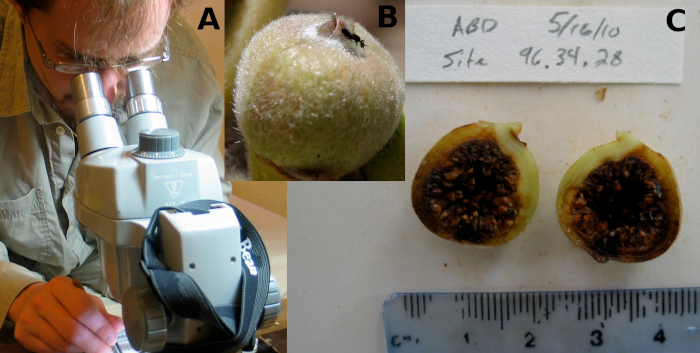
\includegraphics[width=1\linewidth]{img/fig_data_set} \caption{Three images showing the process of collecting data for the dimensions of figs from trees of the Sonoran Desert Rock Fig in Baja, Mexico. (A) Processing fig fruits, which included measuring the diameter of figs along three diferent axes of length, width, and height, (B) a fig still attached to a tree with a fig wasp on top of it, and (C) a sliced open fig with seeds along the inside of it.}\label{fig:unnamed-chunk-3}
\end{figure}

This lab will use the \href{https://raw.githubusercontent.com/bradduthie/statistical_techniques/main/data/soil_organic_carbon.csv}{soil organic carbon} dataset in \protect\hyperlink{02_summary_statistics}{Exercise 8.1} for summary statistics.
The \href{https://raw.githubusercontent.com/bradduthie/statistical_techniques/main/data/fig_fruits.csv}{fig fruits} will be used for \protect\hyperlink{02_transforming_variables}{Exercise 8.2} on transforming variables and \protect\hyperlink{02_computing_variables}{Exercise 8.3} on computing a variable.

\hypertarget{summary_statistics_02}{%
\section{Exercise for summary statistics}\label{summary_statistics_02}}

Download the \href{https://raw.githubusercontent.com/bradduthie/statistical_techniques/main/data/soil_organic_carbon.csv}{soil organic carbon} dataset if you have not already done so, and save it in a location where you know you will be able to find it again, then open Jamovi.
Once Jamovi is open, you can import the dataset by clicking on the three lines in the upper left corner of the tool bar, then selecting `Open' (Figure 8.2).

\begin{figure}
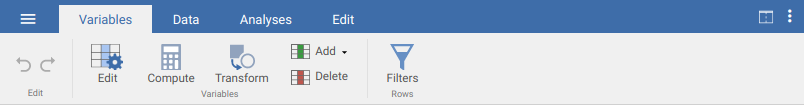
\includegraphics[width=1\linewidth]{img/jamovi_toolbar} \caption{The Jamovi toolbar including tabs for opening files, Variables, Data, Analyses, and Edit. To open a file, select the three horizontal lines in the upper right}\label{fig:unnamed-chunk-5}
\end{figure}

You might need to click `Browse' in the upper right of Jamovi to find the file.
Figure 8.3 below shows how this will look when you browse for a data file.

\begin{figure}
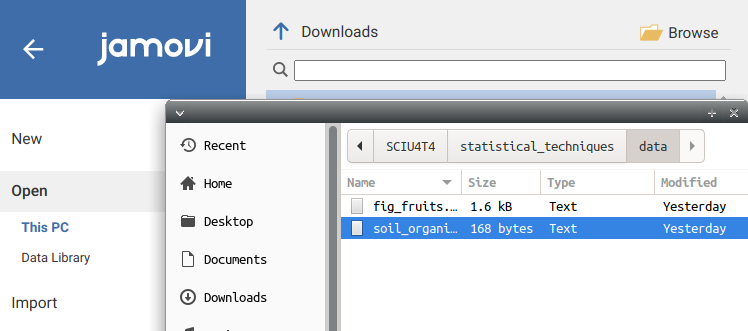
\includegraphics[width=1\linewidth]{img/open_soil_organic_carbon} \caption{The Jamovi interface for opening a file with the 'Import' tab selected. Options for browsing to a file on the computer are available in the upper right, which opens the window in the foreground.}\label{fig:unnamed-chunk-6}
\end{figure}

Once the data are imported, you should see two separate columns.
The first column will show soil organic carbon values for topsoil samples, and the second column will show soil organic carbon values for subsoil samples.
Notice right away that these data are not formatted in a tidy way.
We need to fix this so that each row is a unique sample, and each column represents some property of the sample (see the previous chapter section on \protect\hyperlink{data_organisation}{data organisation} for a reminder of why).
It might be easiest to reorganise the data in a spreadsheet such as LibreOffice Calc or Microsoft Excel.
But you can also edit the directly in Jamovi by clicking on the `Data' tab in the toolbar (see Figure 8.2).
The best way to reorganise the data in Jamovi is to double-click on the third column of data next to `subsoil' (see Figure 8.4).

\begin{figure}
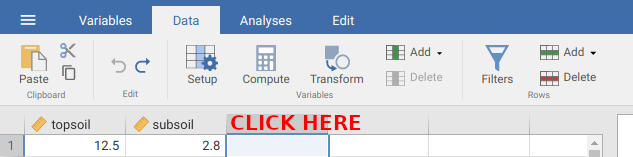
\includegraphics[width=1\linewidth]{img/jamovi_new_variable} \caption{The Jamovi toolbar is shown with the soil organic carbon dataset. In Jamovi, double-clicking above column three where it says 'CLICK HERE' will allow you to input a new variable.}\label{fig:unnamed-chunk-7}
\end{figure}

After double-clicking on the location shown in Figure 8.4, there will be three buttons visible.
You can click the `New Data Variable' to insert a new variable named `soil\_type' in place of the default name `C'.
Keep the `Measure type' as `Nominal', but change the `Data type' to `text'.
When you are done, click the \texttt{\textgreater{}} character to the right so that the variable is fixed (Figure 8.5).

\begin{figure}
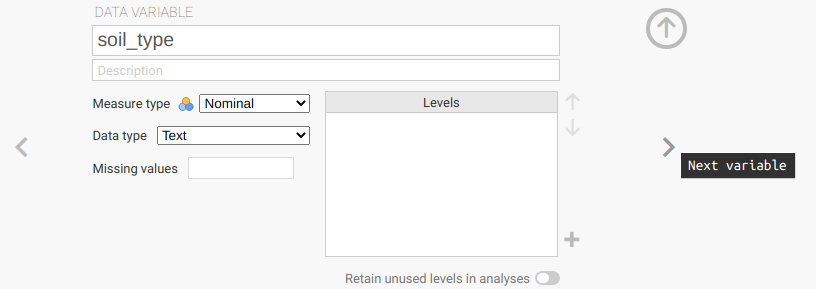
\includegraphics[width=1\linewidth]{img/jamovi_set_variable} \caption{The Jamovi toolbar is shown with the input for creating a new data variable. The new variable added is to indicate the soil type (topsoil or subsoil), so it needs to be a nominal variable with a data type of text.}\label{fig:unnamed-chunk-8}
\end{figure}

After typing in the new variable `soil\_type', add another variable called `organic\_carbon'.
The organic\_carbon variable should have a measure type of `Continuous' and a data type of `Decimal'.
After both soil\_type and organic\_carbon variables have been set, you can click the up arrow with the upper right circle (Figure 8.5) to get the new variable window out of the way.

With the two new variables created, we can now rearrange the data in a tidy way.
The first 19 rows of soil\_type should be `topsoil', and the remaining 15 rows should be `subsoil'.
To do this quickly, you can write `topsoil' in the first row of soil\_type and copy-paste into the remaining rows.
You can do the same to write `subsoil' in the remaining rows 20-34.
Next, copy all of the topsoil values in column 1 into the first 19 rows of column 4, and copy all of the subsoil values in column 2 into the next 15 rows.
After doing all of this, you column 3 (soil\_type) should have the word `topsoil' in rows 1-19 and `subsoil' in rows 20-34.
The values from columns 1 and 2 should now fill rows 1-34 of column 4.
You can now delete the first column of data by right clicking on the column name `topsoil' and selecting `Delete Variable'.
Do the same for the second column `subsoil'.
Now you should have a tidy data set with two columns of data, one called `soil\_type' and one called `organic\_carbon'.
You are now ready to calculate some descriptive statistics from the data.

First, we can calculate the minimum, maximum, and mean of all of the organic carbon values.
To do this, select the `Analyses' tab, then click on the left-most button called `Exploration' in the toolbar (Figure 8.6).

\begin{figure}
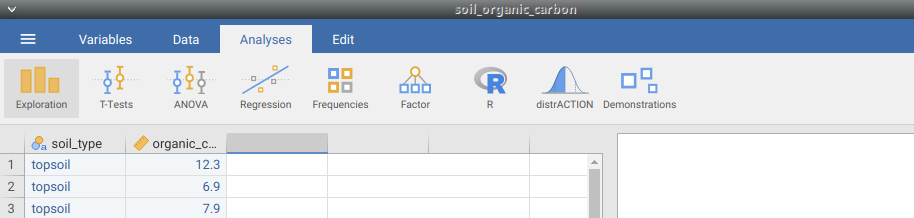
\includegraphics[width=1\linewidth]{img/jamovi_exploration} \caption{The Jamovi toolbar where the tab 'Analyses' can be selected at the very top. Below this tab, the button 'Exploration' can be clicked to calculate descriptive statistics.}\label{fig:unnamed-chunk-9}
\end{figure}

After clicking on `Exploration', a pull-down box will appear with an option for `Descriptives'.
Select this option, and you will see a new window with our two columns of data in the left-most box.
Click once on the `organic\_carbon' variable and use the right arrow to move it into the `Variables' box.
In the right-most panel of Jamovi, a table called `Descriptives' will appear, which will include values for the organic carbon mean, minimum, and maximum.
Write these values on the lines below, and remember to include units.

Mean: \_\_\_\_\_\_\_\_\_\_\_\_\_\_\_\_\_\_\_\_\_\_\_\_\_\_\_\_

Minimum: \_\_\_\_\_\_\_\_\_\_\_\_\_\_\_\_\_\_\_\_\_\_\_\_\_\_\_\_

Maximum: \_\_\_\_\_\_\_\_\_\_\_\_\_\_\_\_\_\_\_\_\_\_\_\_\_\_\_\_

These values might be useful, but recall that there are two different soil types that need to be considered, topsoil and subsoil.
The mean, minimum, and maximum above pools both of these soil types together, but we might instead want to know the mean, minimum, and maximum values for topsoil and subsoil separately.
Splitting organic carbon by soil types is straightforward in Jamovi.
To do it, go back to the Exploration \(\to\) Descriptives option and again put `organic\_carbon' in the Variables box.
This time, however, notice the `Split by' box below the Variables box.
Now, click on `soil\_type' in the descriptives and click on the lower right arrow to move soil type into the `Split by' box.
The table of descriptives in the right window will now break down all of the summary statistics by soil type.
First, write the mean, minimum, and maximum topsoil values below.

Mean: \_\_\_\_\_\_\_\_\_\_\_\_\_\_\_\_\_\_\_\_\_\_\_\_\_\_\_\_

Minimum: \_\_\_\_\_\_\_\_\_\_\_\_\_\_\_\_\_\_\_\_\_\_\_\_\_\_\_\_

Maximum: \_\_\_\_\_\_\_\_\_\_\_\_\_\_\_\_\_\_\_\_\_\_\_\_\_\_\_\_

Next, do the same for the mean, minimum, and maximum subsoil values.

Mean: \_\_\_\_\_\_\_\_\_\_\_\_\_\_\_\_\_\_\_\_\_\_\_\_\_\_\_\_

Minimum: \_\_\_\_\_\_\_\_\_\_\_\_\_\_\_\_\_\_\_\_\_\_\_\_\_\_\_\_

Maximum: \_\_\_\_\_\_\_\_\_\_\_\_\_\_\_\_\_\_\_\_\_\_\_\_\_\_\_\_

From the values above, the mean of organic carbon sampled from the topsoil appears to be greater than the mean of organic carbon sampled from the subsoil.
Assuming that Jamovi has calculated the means correctly, we can be confident that the topsoil sample mean is higher.
But what about the \emph{population} means?
Think back to concepts of populations versus samples from \protect\hyperlink{Chapter_4}{Chapter 4}.
Based on these samples in the dataset, can we really say for certain that the population mean of topsoil is higher than the population mean of subsoil?
Think about this, then write a sentence below about how confident we can be about concluding that topsoil organic carbon is greater than subsoil organic carbon.

\begin{verbatim}




\end{verbatim}

What would make you more (or less) confident that topsoil and subsoil population means are different?
Think about this, then write another sentence below that answers the question.

\begin{verbatim}




\end{verbatim}

Note that there is no right or wrong answer for the above two questions.
The entire point of the questions is to help you reflect on your own learning and better link the concepts of populations and samples to the real dataset in this practical.
Doing this will make the statistical hypothesis testing that comes later in the module more clear.

\hypertarget{transforming_variables_02}{%
\section{Exercise on transforming variables}\label{transforming_variables_02}}

In this next exercise, we will work with the \href{https://raw.githubusercontent.com/bradduthie/statistical_techniques/main/data/fig_fruits.csv}{fig fruits} dataset.
Open this dataset into Jamovi.
Note that there are five columns of data, and all of the data appear to be in a tidy format.
Each row represents a separate fig fruit, while each column represents a measured variable associated with the fruit.
The first several rows should look like the below.

\begin{verbatim}
##   Tree Length_cm Width_cm Height_cm Seeds
## 1    A       1.5      1.8       1.4   238
## 2    A       1.7      1.9       1.5   198
## 3    A       2.1      2.1       1.6   220
## 4    A       1.5      1.6       1.4   188
## 5    A       1.6      1.6       1.5   139
## 6    A       1.5      1.4       1.5   173
\end{verbatim}

The dataset includes the tree from which the fig was sampled in column 1 (A, B, C, and D), then the length, width, and heights of the fig in cm.
Finally, the last column shows how many seeds were counted within the fig.
Use the Descriptives option in Jamovi to find the overall (i.e., not split by Tree) mean length, width, and height of figs in the dataset.
Write these means down below (remember the units).

Mean length: \_\_\_\_\_\_\_\_\_\_\_\_\_\_\_\_\_\_\_\_\_\_\_\_\_\_\_\_

Mean height: \_\_\_\_\_\_\_\_\_\_\_\_\_\_\_\_\_\_\_\_\_\_\_\_\_\_\_\_

Mean width: \_\_\_\_\_\_\_\_\_\_\_\_\_\_\_\_\_\_\_\_\_\_\_\_\_\_\_\_

Now look at the different rows in the Descriptives table of Jamovi.
Note that there is a row for `Missing', and there appears to be one missing value for fig width and fig height.
This is very common in real datasets.
Sometimes practical limitations in the field prevent data from being collected, or something happens that causes data to be lost.
We therefore need to be able to work with datasets that have missing data.
For now, we will just note the missing data and find them in the actual data set.
Go back to the `Data' tab in Jamovi and find the figs with a missing width and height value.
Report the rows of these missing values below.

Missing width row: \_\_\_\_\_\_\_\_\_\_\_\_\_\_\_\_\_\_\_\_\_\_\_\_\_\_\_\_

Missing height row: \_\_\_\_\_\_\_\_\_\_\_\_\_\_\_\_\_\_\_\_\_\_\_\_\_\_\_\_

Next, we will go back to working with the actual data.
Note that the length, width, and height variables are all recorded in cm to a single decimal place.
Suppose we want to transform these variables so that they are represented in mm instead of cm.
We will start by creating a new column `Length\_mm' by transforming the existing `Length\_cm' column.
To do this, click on the `Data' tab at the top of the toolbar again, then click on the `Length\_cm' column name to highlight the entire column.
Your screen should look like the image in Figure 8.7.

\begin{figure}
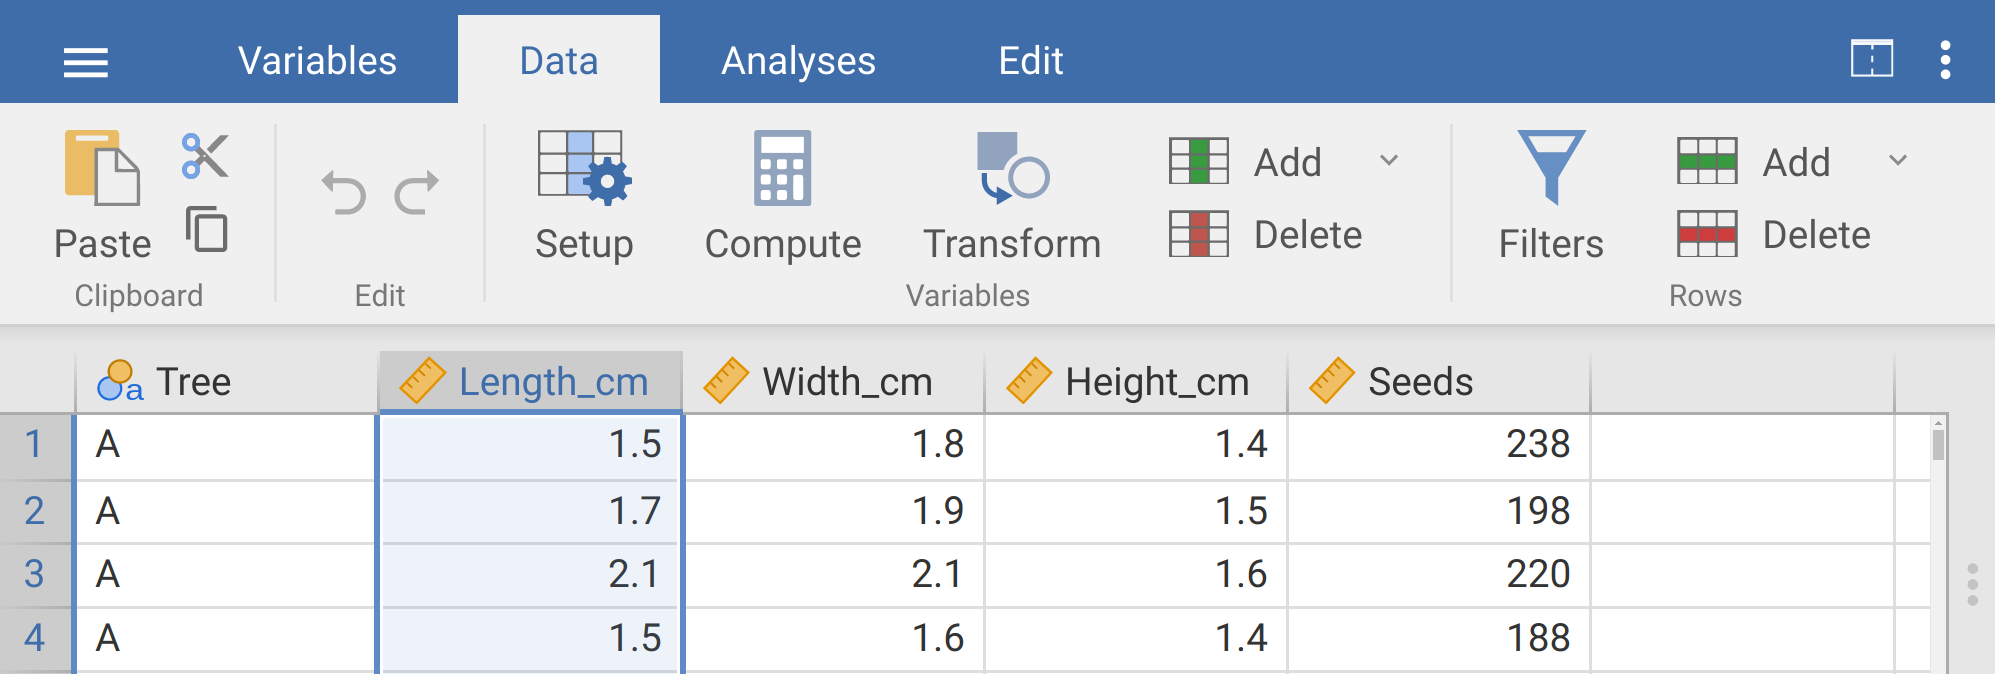
\includegraphics[width=1\linewidth]{img/jamovi_transform_fig_length} \caption{The Jamovi toolbar where the tab 'Data' is selected. The length (cm) column is highlighted and will be transformed by clicking on the Transform button in the toolbar above}\label{fig:unnamed-chunk-11}
\end{figure}

With the `Length\_cm' column highlighted, click on the `Transform' button in the toolbar.
Two things happen next.
First, a new column appears in the dataset that looks identical to `Length\_cm'; ignore this for now.
Second, a box appears below the toolbar allowing us to type in a new name for the transformed variable.
We can call this variable `Length\_mm'.
Below, note the first pulldown menu `Source variable'.
The source value should be `Length\_cm', so we can leave this alone.
The second pulldown menu `using transform' will need to change.
To change the transform from `None', click the arrow and select `Create New Transform' from the pulldown.
A new box will pop up allowing us to name the transformation.
It does not matter what we call it (e.g., `cm\_to\_mm' is fine).
Note that there are 10 mm in 1 cm, so to convert from cm to mm, we need to multiply the values of `Length\_cm' by 10.
We can do this by appending a \texttt{*\ 10} to the lower box of the transform window, so that it reads \texttt{=\ \$source\ *\ 10} (Figure 8.8).

\begin{figure}
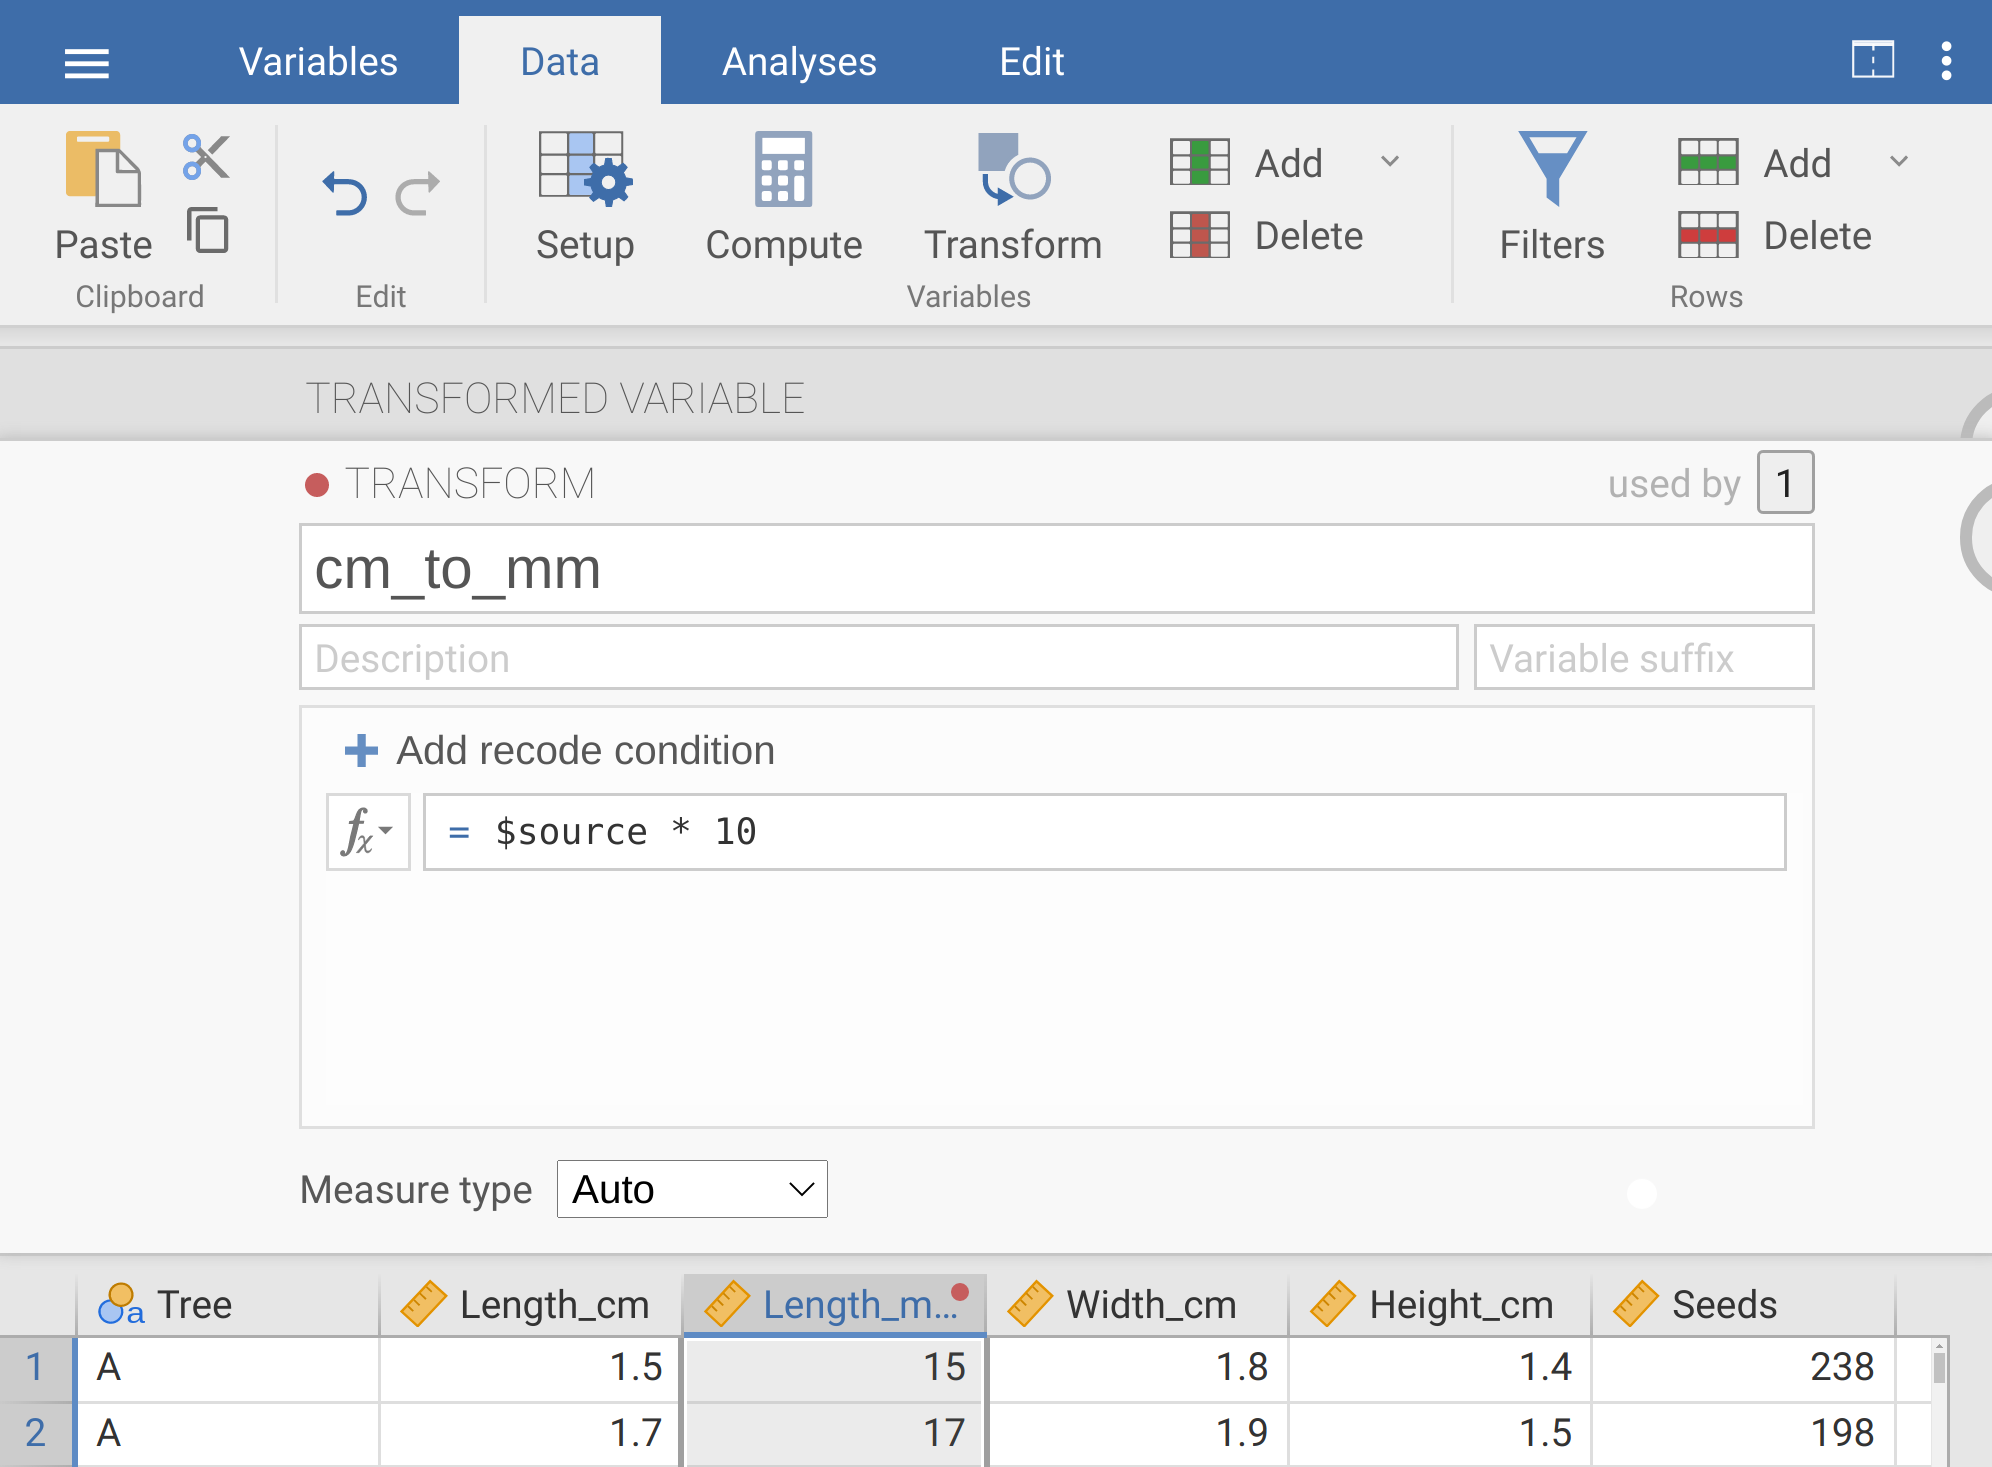
\includegraphics[width=1\linewidth]{img/jamovi_transform_cm_to_mm} \caption{The Jamovi toolbar where the tab 'Data' is selected. The box below shows the transform, which has been named 'cm to mm'. The transformation occurs by multiplying the source (Length mm) by 10. The dataset underneath shows the first few rows with the transformed column highlighted (note that the new 'Length mm' column is 10 times the length column.}\label{fig:unnamed-chunk-12}
\end{figure}

When we are finished, we can click the down arrow inside the circle in the upper right to get rid of the transform window, then the up arrow inside the circle in the upper right to get rid of the transformed variable window.
Now we have a new column called `Length\_mm', in which values are 10 times greater than they are in the adjacent `Length\_cm' column, and therefore represent fig length in mm.
If we want to, we can always change the transformation by double-clicking the `Length\_mm' column.
For now, apply the same transformation to fig width and height, so we have three new columns of length, width, and height all measured in mm (note, if you want to, you can use the saved transformation `cm\_to\_mm' that you used to transform length, saving some time).
At the end of this, you should have eight columns of data, including three new columns that you just created by transforming the existing columns of Length\_cm, Width\_cm, and Height\_cm into the new columns Length\_mm, Width\_mm, and Height\_mm.
Find the means of these three new columns and write them below.

Mean length: \_\_\_\_\_\_\_\_\_\_\_\_\_\_\_\_\_\_\_\_\_\_\_\_\_\_\_\_

Mean height: \_\_\_\_\_\_\_\_\_\_\_\_\_\_\_\_\_\_\_\_\_\_\_\_\_\_\_\_

Mean width: \_\_\_\_\_\_\_\_\_\_\_\_\_\_\_\_\_\_\_\_\_\_\_\_\_\_\_\_

Compare these means to the means calculated above in cm.
Do the differences between means in cm and the means in mm make sense?

\hypertarget{computing_variables_02}{%
\section{Exercise on computing variables}\label{computing_variables_02}}

In this last exercise, we will compute a new variable `fig\_volume'.
Because of the way that the dimensions of the fig were measured in the field, we need to make some simplifying assumptions when calculating volume.
We will assume that fig fruits are perfect spheres, and that the radius of each fig is half of its measured width (i.e., `Width\_mm / 2').
This is obviously not ideal, but sometimes practical limitations in the field make it necessary to make these kinds of simplifying assumptions.
In this case, how might assuming that figs are perfectly spherical affect the accuracy of our estimated fig volume?
Write a sentence of reflection on this question below, drawing from what you have learned this week about accuracy and precision of measurements.

\begin{verbatim}




\end{verbatim}

Now we are ready to make our calculation of fig volume.
The formula for the volume of a sphere (\(V\)) given its radius \(r\) is,

\[V = \frac{4}{3} \pi r^{3}.\]

In words, sphere volume equals four thirds times \(\pi\), times \(r\) cubed (i.e., to the third power).
If this equation is confusing, remember that \(\pi\) is approximately 3.14, and taking \(r\) to the third power means that we are multiplying \(r\) by itself 3 times.
We could therefore rewrite the equation above,

\[V = \frac{4}{3} \times 3.14 \times r \times r \times r.\]

This is the formula that we can use to create our new column of data for fig volume.
To do this, click on the first empty column of the dataset, just to the right of the `Seeds' column header.
You will see a pull down option in Jamovi with 3 options, one of which is `NEW COMPUTED VARIABLE'.
This is the option that we want.
We need to name this new variable, so we can call it `fig\_volume'.
Next, we need to type in the formula for calculating volume.
First, in the small box next to the \(f_{x}\), type in the (4/3) multiplied by 3.14 as below.

\begin{verbatim}
= (4/3) * 3.14 *
\end{verbatim}

Next, we need to multiply by the variable `Width\_mm' divided by 2 (to get the radius), three times. We can do this by clicking on the \(f_{x}\) box to the left.
Two new boxes will appear; the first is named `Functions', and the second is named `Variables'.
Ignore the functions box for now, and find `Width\_mm' in the list of variables.
Double click on this to put it into the formula, then divide it by 2.
You can repeat this two more times to complete the computed variable as shown in Figure 8.9.

\begin{figure}
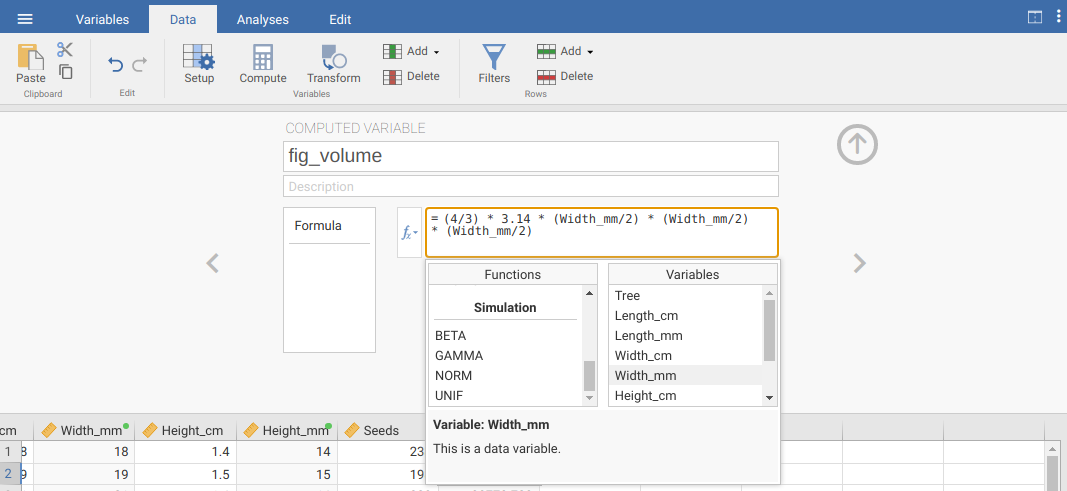
\includegraphics[width=1\linewidth]{img/jamovi_compute_new_variable} \caption{The Jamovi toolbar where the tab 'Data' is selected. The box below shows the new computed variable 'fig volume', which has been created by calculating the product of 4/3, 3.14, and Width mm three times.}\label{fig:unnamed-chunk-13}
\end{figure}

Note that we can get the cube of `Width\_mm' more concisely by using the carrot character (\texttt{\^{}}).
That is, we would get the same answer shown in Figure 8.9 if we instead typed the below in the function box.

\begin{verbatim}
= (4/3) * 3.14 * (Width_mm/2)^3
\end{verbatim}

Note that the order of operations is important here, which is why there are parentheses around \texttt{Width\_mm/2}. This calculation needs to be done before taking the value to the power of 3. If we instead had written, \texttt{Width\_mm/2\^{}3}, the Jamovi would first take the cube of 2 \((2 \times 2 \times 2 = 8)\), then divided \texttt{Width\_mm} by this value giving a different and incorrect answer. When in doubt, it is always useful to use parentheses to specify what calculations should be done first.

You now have the new column of data `fig\_volume'.
Remember that the calculations underlying this new variable need to be done for the units.
The width of the fig was calculated in mm, but we have taken width to the power of 3 when calculating the volume.
In the spaces below, find the overall mean, minimum, and maximum volumes of figs and report them in the correct units.

Mean: \_\_\_\_\_\_\_\_\_\_\_\_\_\_\_\_\_\_\_\_\_\_\_\_\_\_\_\_

Minimum: \_\_\_\_\_\_\_\_\_\_\_\_\_\_\_\_\_\_\_\_\_\_\_\_\_\_\_\_

Maximum: \_\_\_\_\_\_\_\_\_\_\_\_\_\_\_\_\_\_\_\_\_\_\_\_\_\_\_\_

Finally, it would be good to plot these newly calculated fig volume data.
These data are continuous, so we can use a histogram to visualise the fig volume distribution.
To make a histogram, go to the Exploration \(\to\) Descriptives window in Jamovi (the same place where you found the mean, minimum, and maximum).
Now, look on the lower left-hand side of the window and find the pulldown menu for `Plots'.
Click `Plots', and you should see several different plotting options.
Check the option for `Histogram' and see the new histogram plotted in the window to the right.
Draw a rough sketch of the histogram in the area below.

\begin{verbatim}






\end{verbatim}

\hypertarget{part-summary-statistics}{%
\part{Summary statistics}\label{part-summary-statistics}}

\hypertarget{week-3-overview}{%
\chapter*{Week 3 Overview}\label{week-3-overview}}
\addcontentsline{toc}{chapter}{Week 3 Overview}

\begin{longtable}[]{@{}
  >{\raggedright\arraybackslash}p{(\columnwidth - 2\tabcolsep) * \real{0.3269}}
  >{\raggedright\arraybackslash}p{(\columnwidth - 2\tabcolsep) * \real{0.6731}}@{}}
\toprule
\endhead
\textbf{Dates} & 6 February 2023 - 10 February 2023 \\
\textbf{Reading} & \textbf{Required:} SCIU4T4 Workbook chapters 9-12 \\
& \textbf{Recommended:} \citet{Navarro2022} \href{https://davidfoxcroft.github.io/lsj-book/drawing-graphs.html}{Chapter 5} and \href{https://davidfoxcroft.github.io/lsj-book/descriptive-statistics.html\#measures-of-central-tendency}{Chapter 4.1} \\
& \textbf{Optional:} \citet{Rowntree2018} Chapter 3 \\
\textbf{Lectures} & 3.0: Decimal places and significant figures part 1 (8 min.) \\
& 3.1: Decimal places and significant figures part 2 (7 min.) \\
& 3.2: Graphs (11 min.) \\
& 3.3: Box-whisker plots (8 min.) \\
& 3.4: The mean (17 min.) \\
& 3.5: The mode (7 min.) \\
& 3.6: The median and quantiles (8 min.) \\
& 3.7: Mean, mode, median, and resistance (9 min.) \\
\textbf{Practical} & Plotting and statistical summaries \\
\textbf{Assessments} & Week 3 Practice quiz on Canvas \\
\bottomrule
\end{longtable}

\hypertarget{Chapter_9}{%
\chapter{Decimal places, significant figures, and rounding}\label{Chapter_9}}

When making calculations, it is important that any numbers reported are communicated with \protect\hyperlink{Chapter_6}{accuracy and precision}.
This means reporting numbers with the correct number of digits.
This chapter focuses on correctly interpreting the decimal places and significant figures of a number, and correctly rounding.
In your assessments, you will frequently be asked to report an answer to a specific number of decimal places or significant figures, and you will be expected to round numbers correctly.

\hypertarget{decimal-places-and-significant-figures}{%
\section{Decimal places and significant figures}\label{decimal-places-and-significant-figures}}

A higher number of digits communicates a greater level of accuracy
For example, the number 2.718 expresses a higher precision than 2.7 does.
Reporting 2.718 implies that we know the value is somewhere between 2.7175 and 2.1785, but reporting 2.7 only implies that we know the value is somewhere between 2.65 and 2.75 \citep{Sokal1995}.
These numbers therefore have a different number of \emph{decimal places} and a different number \emph{significant figures}.
Decimal places and significant figures are related, but not the same.

\textbf{Decimal places} are conceptually easier to understand. These are just the number of digits to the right of the decimal point. For example, 2.718 has 3 decimal places and 2.7 has 1 decimal place.

\textbf{Significant figures} are a bit more challenging. These are the number of digits that you need to infer the accuracy of a value. For example, the number 2.718 has 4 significant figures and 2.7 has 2 significant figures. This sounds straightforward, but it can get confusing when numbers start or end with zeros. For example, the number 0.045 has only two significant figures because the first two zeros only serve as placeholders (note that if this were a measurement of 0.045 m, then we could express the exact same value as 45 mm, so the zeros are not really necessary to indicate measurement accuracy). In contrast, the measurement 0.045000 has 5 significant figures because the last 3 zeros indicate a higher degree of accuracy than just 0.045 would (i.e., we know the value is somewhere between 0.44995 and 0.45005, not just 0.0445 and 0.0455). Lastly, the measurement 4500 has only 2 significant figures because the last 2 zeros are only serving as a placeholder to indicate magnitude, not accuracy (if we wanted to represent 4500 with 4 significant figures, we could use scientific notation and express it as \(4.500 \times 10^3\)).

Here is a table with some examples of some numbers, their decimal places, and their significant figures.

\begin{longtable}[]{@{}lll@{}}
\caption{Numbers are presented in rows of the first column. Decimal places and significant figures for each row number are presented in the second and third column, respectively.}\tabularnewline
\toprule
Number & Decimal places & Significant figures \\
\midrule
\endfirsthead
\toprule
Number & Decimal places & Significant figures \\
\midrule
\endhead
3.14159 & 5 & 5 \\
0.0333 & 4 & 3 \\
1250 & 0 & 3 \\
50000.0 & 1 & 6 \\
0.12 & 2 & 2 \\
1000000 & 0 & 1 \\
\bottomrule
\end{longtable}

It is a good idea to double-check that the values in these tables make sense.
For assessments, make sure that you are confident that you can report your answer to a given number of decimal places or significant figures.

\hypertarget{rounding}{%
\section{Rounding}\label{rounding}}

Often if you are asked to report a number to a specific number of decimals or significant figures, you will need to round the number.\\
Rounding reduces the number of significant digits in a number, which might be necessary if a number that we calculate has more significant digits than we are justified in expressing.
There are different rules for rounding numbers, but in this module, we will follow \citet{Sokal1995}.
When rounding to the nearest decimal, the last decimal written should not be changed if the number that immediately follows is 0, 1, 2, 3, or 4.
If the number that immediately follows is 5, 6, 7, 8, or 9, then the last decimal written should be increased by 1.

For example, if we wanted to round the number 3.141593 to 2 significant digits, then we would write it as 3.1 because the digit that immediately follows (i.e., the third digit) is 4.
If we wanted to round the number to 5 significant digits, then we would write it as 3.1415 because the digit that immediately follows is 9.
And if we wanted to round 3.141593 to 4 significant digits, then we would write it as 3.146 because the digit that immediately follows is 5.
Note that this does not just apply for decimals.
If we wanted to round 1253 to 3 significant figures, then we would round by writing it as 1250.

Here is a table with some examples of numbers rounded to a given significant figure.

\begin{longtable}[]{@{}lll@{}}
\caption{Numbers to be rounded are presented in rows of the first column. The significant figures to which rounding is desired is in the second column, and the third column shows the correctly rounded number.}\tabularnewline
\toprule
Original number & Significant figures & Rounded number \\
\midrule
\endfirsthead
\toprule
Original number & Significant figures & Rounded number \\
\midrule
\endhead
23.2439 & 4 & 23.24 \\
10.235 & 4 & 10.24 \\
102.39 & 2 & 100 \\
5.3955 & 3 & 5.40 \\
37.449 & 3 & 37.4 \\
0.00345 & 2 & 0.0035 \\
\bottomrule
\end{longtable}

In this module, it will be necessary to round calculated values to specified decimal or significant figure.
It is therefore important to understand the rules for rounding and why the values in the table above are rounded correctly.

\hypertarget{Chapter_10}{%
\chapter{Graphs}\label{Chapter_10}}

Graphs are useful tools for visualising and communicating data.
Graphs come in many different types, and different types of graphs are effective for different types of data.
This chapter focuses on four types of graphs: (1) histograms, (2) pie charts, (3) barplots, and (4) box-whisker plots.

After collecting or obtaining a new dataset, it is almost always a good idea to plot the data in some way.
Visualising a dataset can often highlight important and obvious properties of a dataset more efficiently that inspecting raw data, calculating summary statistics, or running statistical tests.
When making graphs to communicate data visually, it is important to ensure the person reading the graph has a clear understanding what is being presented.
In practice, this means clearly labelling axes with meaningful descriptions and appropriate units, including a descripting caption, and indicating what any graph symbols mean.
In general, it is also best to make the simplest graph possible for visualising the data, which means avoiding unnecessary colour, three-dimensional display, or unnecessary distractions from the information being conveyed \citep{Dytham2011, Kelleher2011}.
It is also important to ensure that graphs are as accessible as possible, e.g., by providing strong colour contrast and appropriate colour combinations \citep{Elavsky2022}, and alternative text for images where possible.
As a guide, the histogram, pie chart, barplot, and box-whisker plot below illustrate good practice when making graphs.

\hypertarget{histograms}{%
\section{Histograms}\label{histograms}}

Histograms illustrate the distribution of \protect\hyperlink{Chapter_5}{continuous data}.
They are especially useful visualisation tools because it is often important to assess data at a glance and make a decision about how to proceed with a statistical analysis.
The histogram shown in Figure 10.1 provides an example from the \href{https://raw.githubusercontent.com/bradduthie/statistical_techniques/main/data/fig_fruits.csv}{fig fruits} data set from the practical in \protect\hyperlink{Chapter_8}{Chapter 8}.

\begin{figure}
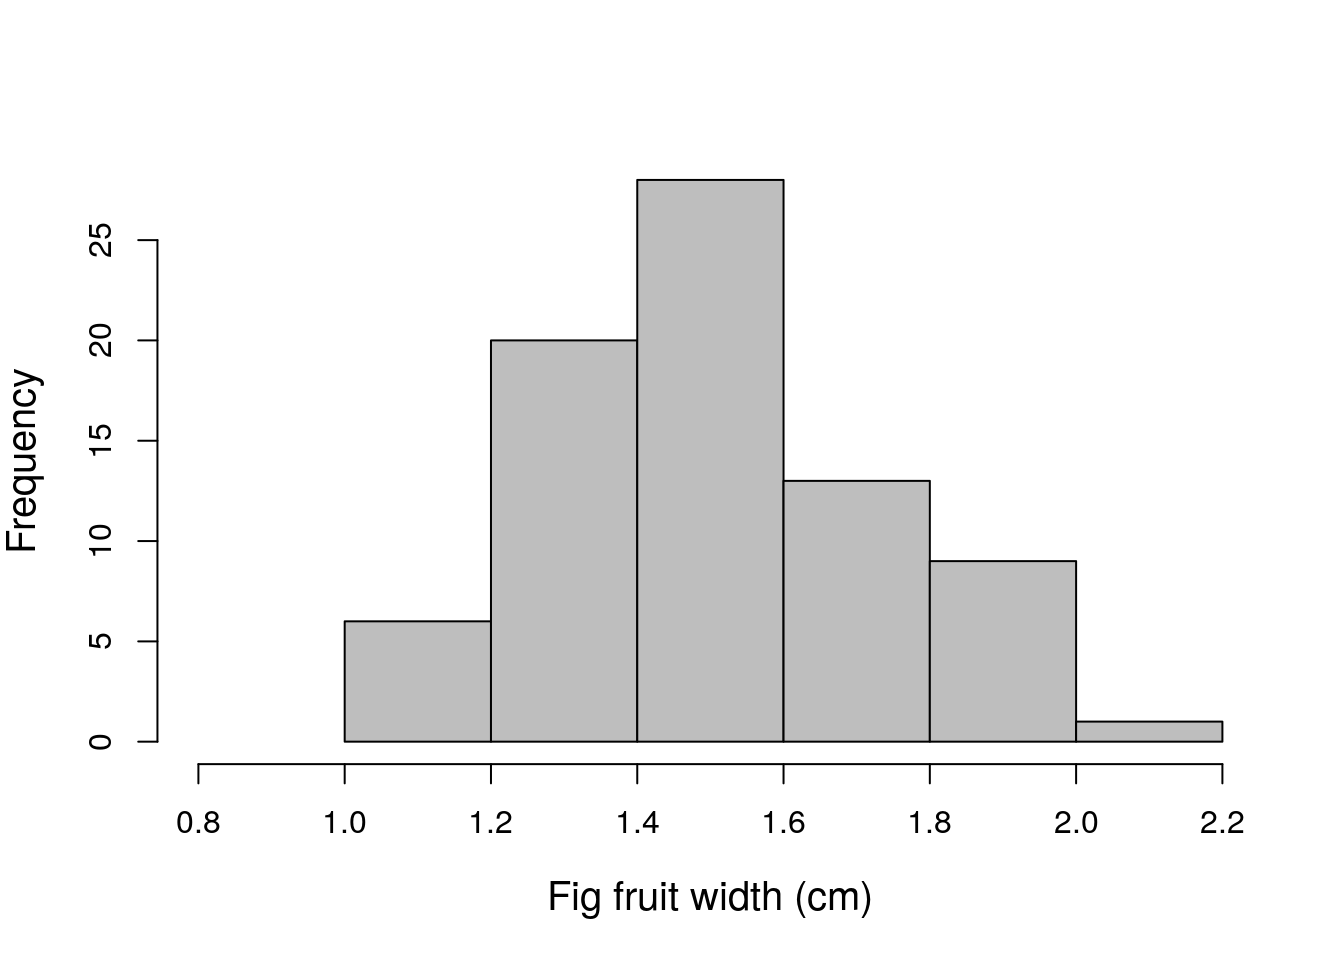
\includegraphics[width=1\linewidth]{bookdown-demo_files/figure-latex/unnamed-chunk-14-1} \caption{Example histogram fig fruit width (cm) using data from 78 fig fruits collected in in 2010 from Baja, Mexico.}\label{fig:unnamed-chunk-14}
\end{figure}

The histogram in Figure 10.1 shows how many fruits there are for different intervals of width (for a step-by-step demonstration of how a histogram is built, see \href{https://bradduthie.shinyapps.io/build_histogram/}{this interactive application}\footnote{Here is the full URL: \url{https://bradduthie.shinyapps.io/build_histogram/}.}).
That is, the frequency with which fruits within some width interval occur in the data.
For example, there are 6 fruits with a width between 1.0 and 1.2, so for this interval on the x-axis, the bar is 6 units in height on the y-axis.
In contrast, there is only 1 fig fruit that has a width greater than 2.0 cm (the biggest is 2.1 cm), so we see that the height of the bar for the interval between 2.0 and 2.2 is only 1 unit in frequency.
The bars of the histogram touch each other, which reinforces that the data are \protect\hyperlink{Chapter_5}{continuous} \citep{Dytham2011, Sokal1995}.

It is especially important to be able to read and understand information from a histogram because it is often necessary to determine if the data are consistent with the assumptions of a statistical test.
For example, the \emph{shape} of the distribution of fig fruit widths might be important for performing a particular test.
For the purposes of this module, the \emph{shape} of the distribution just means what the data look like when plotted like this in a histogram.
In this case, there is a peak toward the centre of the distribution, with fewer low and high values (this kind of distribution is quite common).
Different distribution shapes will be discussed more in Part IV (next week).

\hypertarget{barplots-and-pie-charts}{%
\section{Barplots and pie charts}\label{barplots-and-pie-charts}}

While histograms are an effective way of visualising \protect\hyperlink{Chapter_5}{continuous data}, barplots (also known as `bar charts' or `bar graphs') and pie charts can be used to visualise \protect\hyperlink{Chapter_5}{categorical data}.
For example, in the \href{https://raw.githubusercontent.com/bradduthie/statistical_techniques/main/data/fig_fruits.csv}{fig fruits} data set \protect\hyperlink{Chapter_8}{Chapter 8}, 78 fig fruits were collected from 4 different trees (A, B, C, and D).
A barplot could be used to show how many samples were collected from each tree (see Figure 10.2).

\begin{figure}
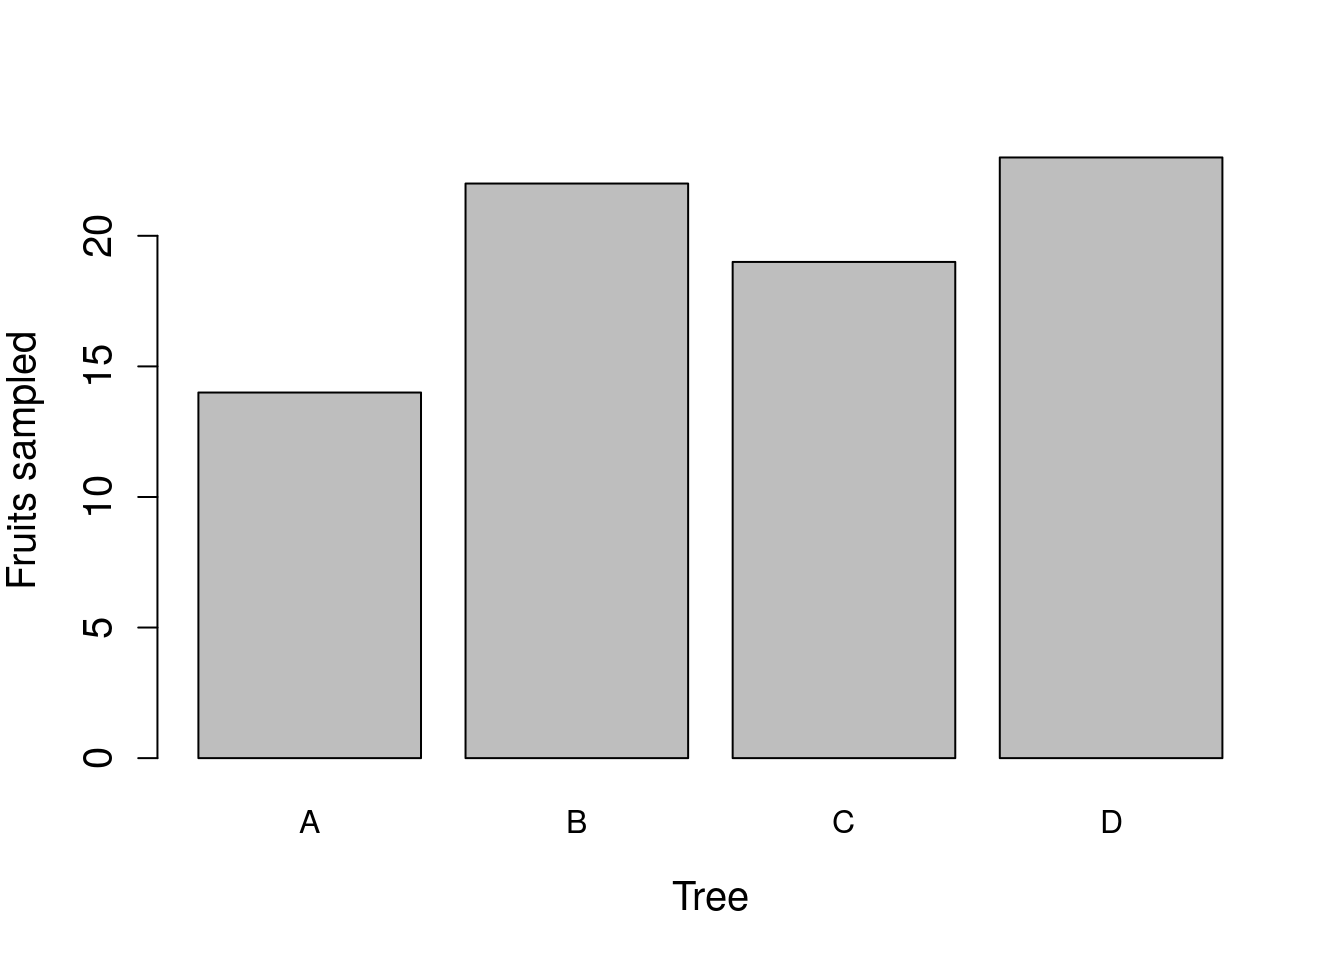
\includegraphics[width=1\linewidth]{bookdown-demo_files/figure-latex/unnamed-chunk-15-1} \caption{Example bar plot showing how many fruits were collected from each of 4 trees (78 collected in total) in 2010 from Baja, Mexico.}\label{fig:unnamed-chunk-15}
\end{figure}

In Figure 10.2, each tree is represented by a separate bar on the x-axis.
Unlike a histogram, the bars do not touch each other, which reinforces that different categories of data are being shown (in this case, different trees).
The height of bar indicates how many fruits were sampled for each tree.
For example, 14 fruits were sampled from tree A, and 22 fruits were sampled from tree B.
At a glance, it is therefore possible to compare different trees and make inferences about how they differ in sampled fruits.

Pie charts are similar to barplots in that both present categorical data, but pie charts are more effective for visualising the relative quantity for each category.
That is, pie charts illustrate the percentage of measurements for each category.
For example, in the case of the fig fruits, it might be useful to visualise what percentage of fruits were sampled from each tree.
A pie chart could be used to evaluate this, with pie slices corresponding to different trees and the size of each slice reflecting the percentage of the total sampled fruits that came from each tree (Figure 10.3).

\begin{figure}
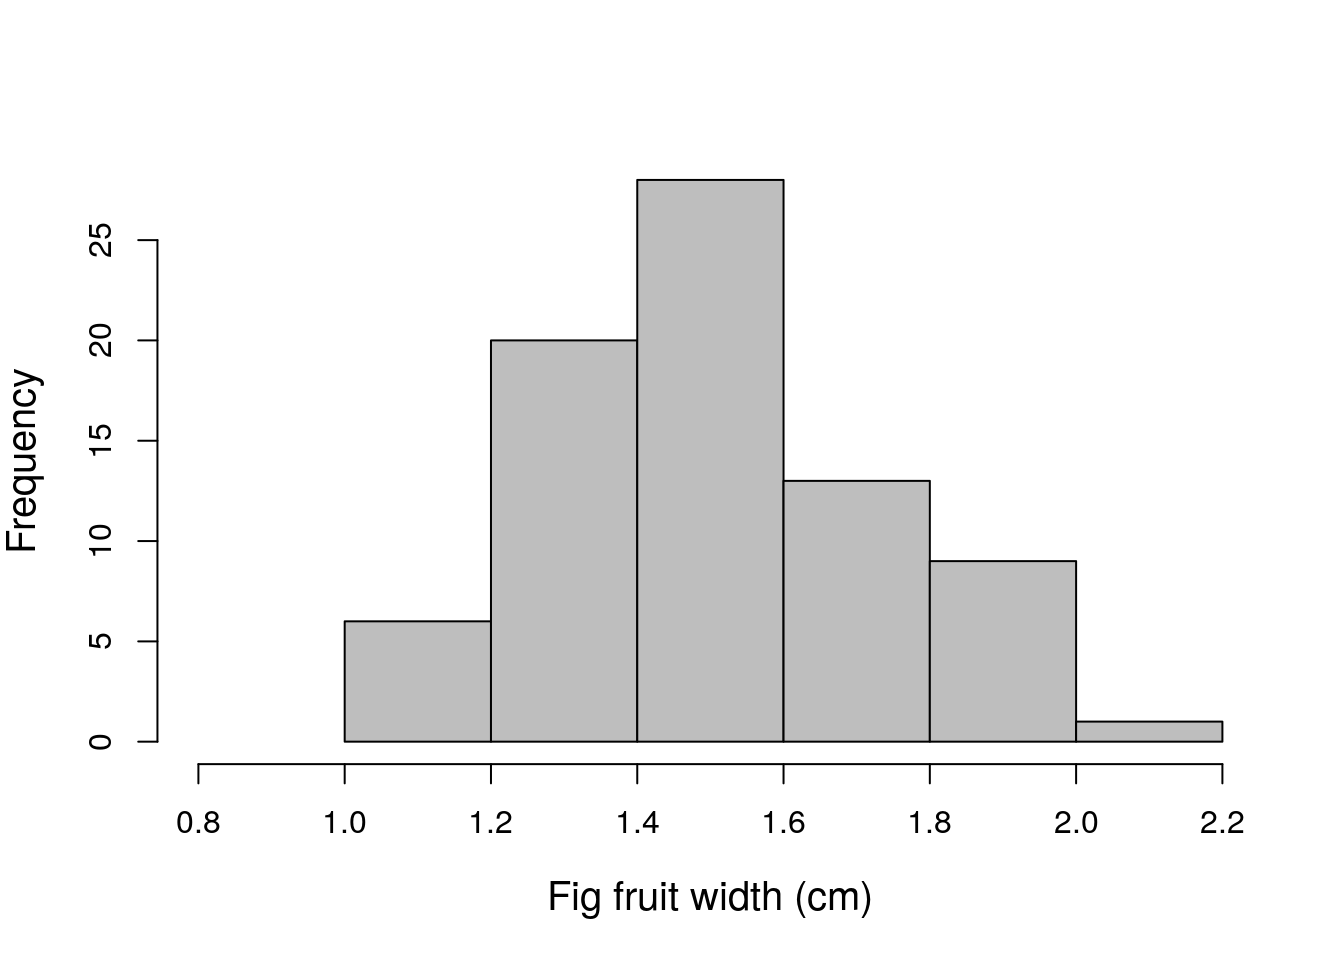
\includegraphics[width=1\linewidth]{bookdown-demo_files/figure-latex/unnamed-chunk-16-1} \caption{Example pie plot showing the percentage of fruits that were collected from each of 4 trees (78 collected in total) in 2010 from Baja, Mexico.}\label{fig:unnamed-chunk-16}
\end{figure}

Pie charts can be useful in some situations, but in the biological and environmental they are not used as often as barplots.
In contrast to pie charts, barplots present the absolute quantities (in Figure 10.2, e.g., the actual number of fruits sampled per tree), and it is still possible with barplots to infer the percentage each category contributes to the total from the relative sizes of the bars.
Pie charts, in contrast, only illustrate relative percentages unless numbers are used to indicate absolute quantities.
Unless only percentage is important, barplots are often the preferred way to communicate count data.

\hypertarget{box-whisker-plots}{%
\section{Box-whisker plots}\label{box-whisker-plots}}

Box-whisker plots (also called boxplots) can be used to visualise distributions in a different way than histograms.
Instead of presenting the full distribution, as in a histogram, a box-whisker plot shows where summary statistics are located (summary statistics are explained below).
This allows the distribution of data to be represented in a more compact way, but does not show the full shape of a distribution.
Figure 10.4 compares a box-whisker plot of fig fruit widths (10.4A) with a histogram of fig fruit widths (10.4B).
In other words, both of the panels (A and B) in Figure 10.4 show the same information in two different ways (note that these are the same data as presented in Figure 10.1).

\begin{figure}
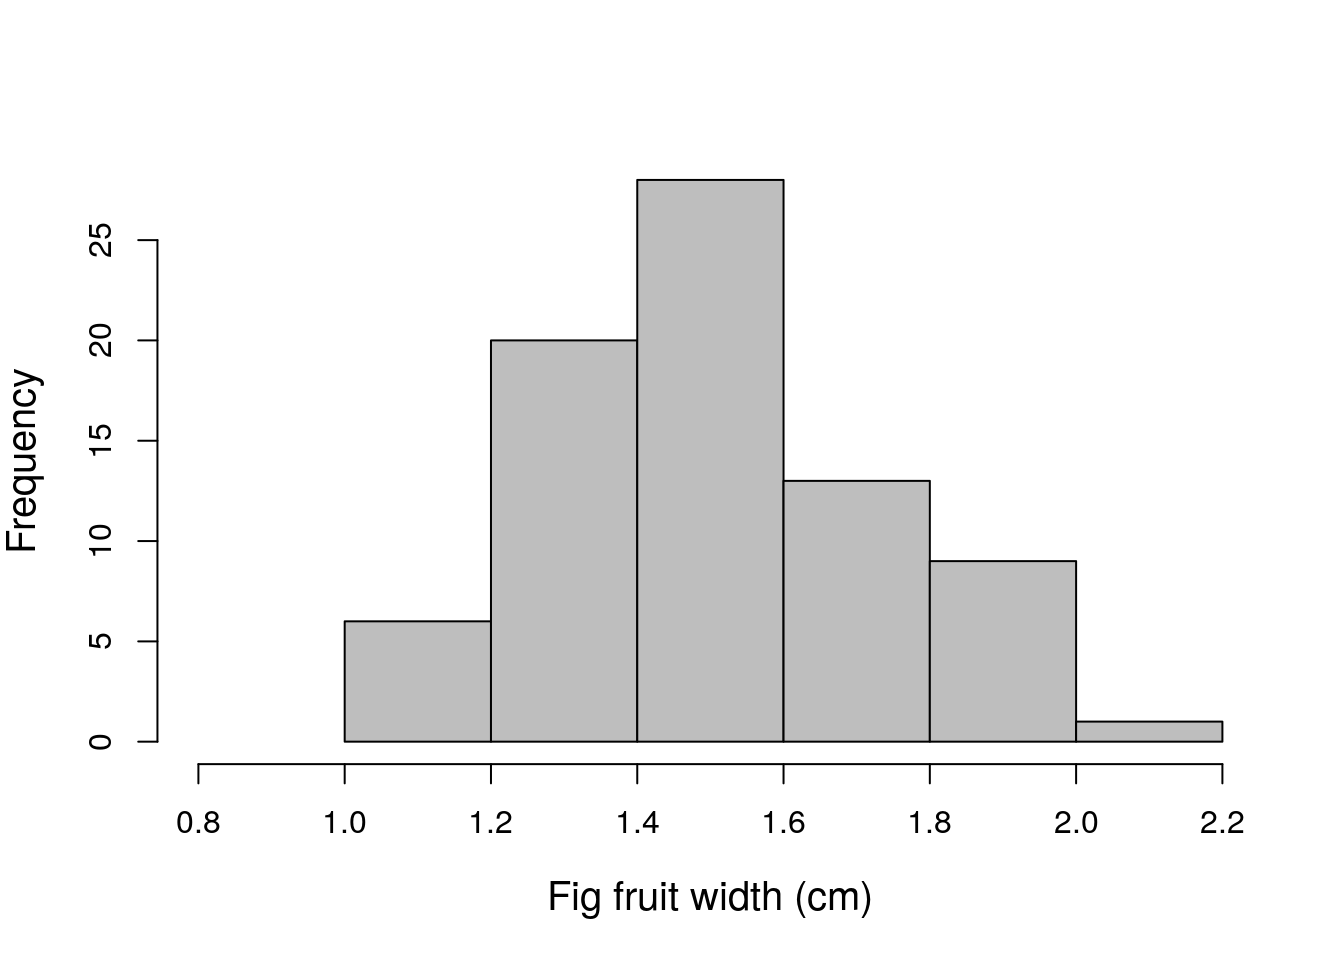
\includegraphics[width=1\linewidth]{bookdown-demo_files/figure-latex/unnamed-chunk-17-1} \caption{Boxplot (A) of fig fruit widths (cm) for 78 fig fruits collected in 2010 in Baja, Mexico. Panel (B) presents the same data as a histogram.}\label{fig:unnamed-chunk-17}
\end{figure}

To show how the panels of Figure 10.4 correspond to one another more clearly, Figure 10.5 shows them again, but with points indicating where the summary statistics shown in the boxplot (Figure 10.5A) are located in the histogram (Figure 10.5B).
These summary statistics include the median (black circles of Figure 10.5), quartiles (red squares of Figure 10.5), and the limits of the distribution (i.e., the minimum and maximum values; blue triangles of Figure 10.5).
Note that in boxplots, if outliers exist, they are presented as separate points.

\begin{figure}
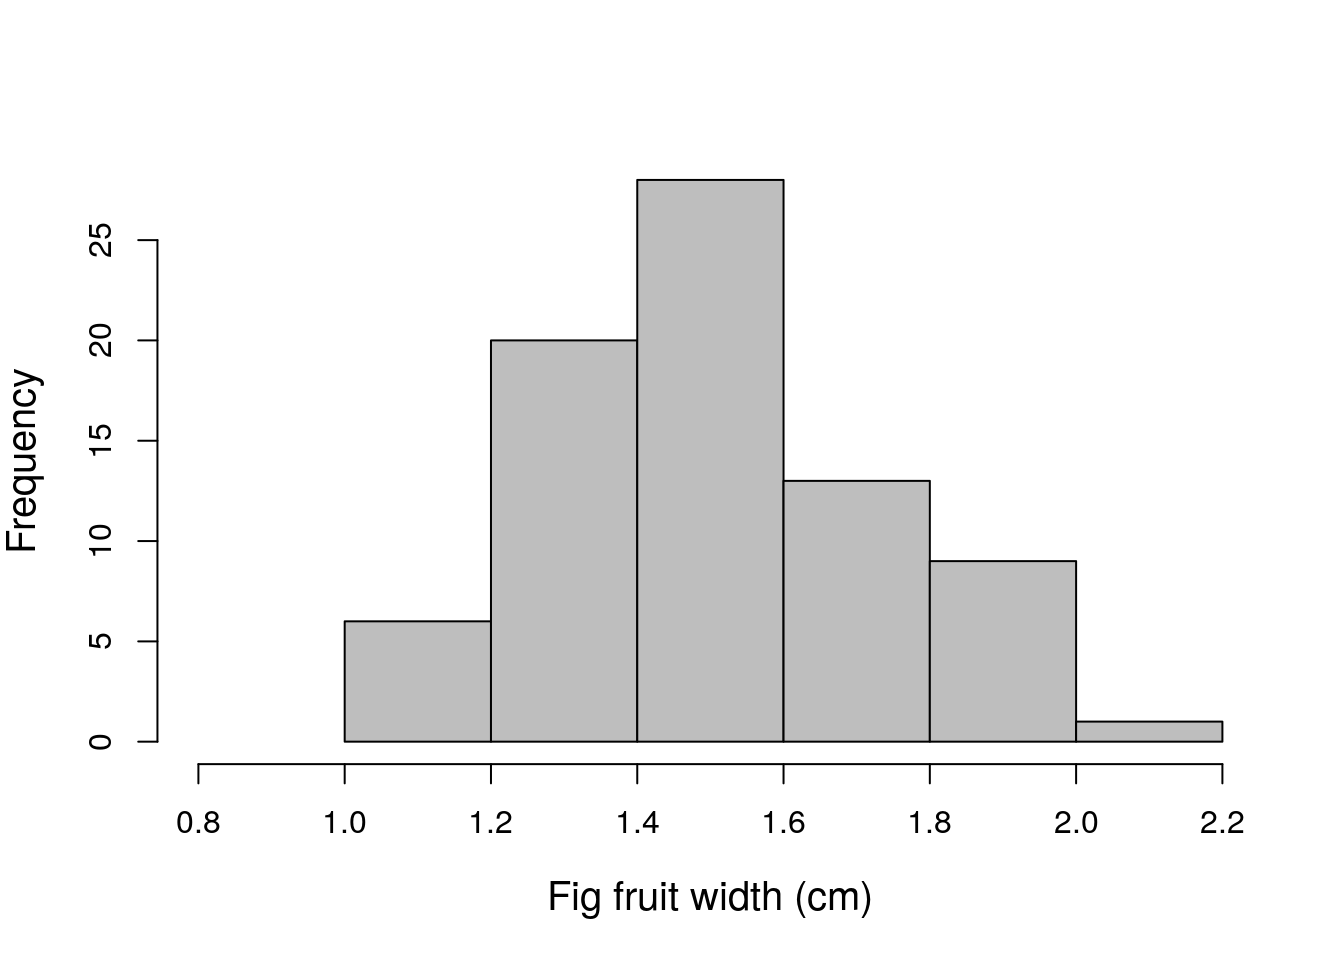
\includegraphics[width=1\linewidth]{bookdown-demo_files/figure-latex/unnamed-chunk-18-1} \caption{Boxplot (A) of fig fruit widths (cm) for 78 fig fruits collected in 2010 in Baja, Mexico. Panel (B) presents the same data as a histogram. Points in the boxplot indicate the median (black circle), first and third quartiles (red squares), and the limits of the distribution (blue triangles). Corresponding locations are shown on the histogram in panel (B).}\label{fig:unnamed-chunk-18}
\end{figure}

One benefit of a boxplot is that it is possible to show the distribution of multiple variables simultaneously.
For example, the distribution of fig fruit width can be shown for each of the four trees side by side on the same x-axis of a boxplot (Figure 10.6).
While it is possible to show histograms side by side, it will quickly take up a lot of space.

\begin{figure}
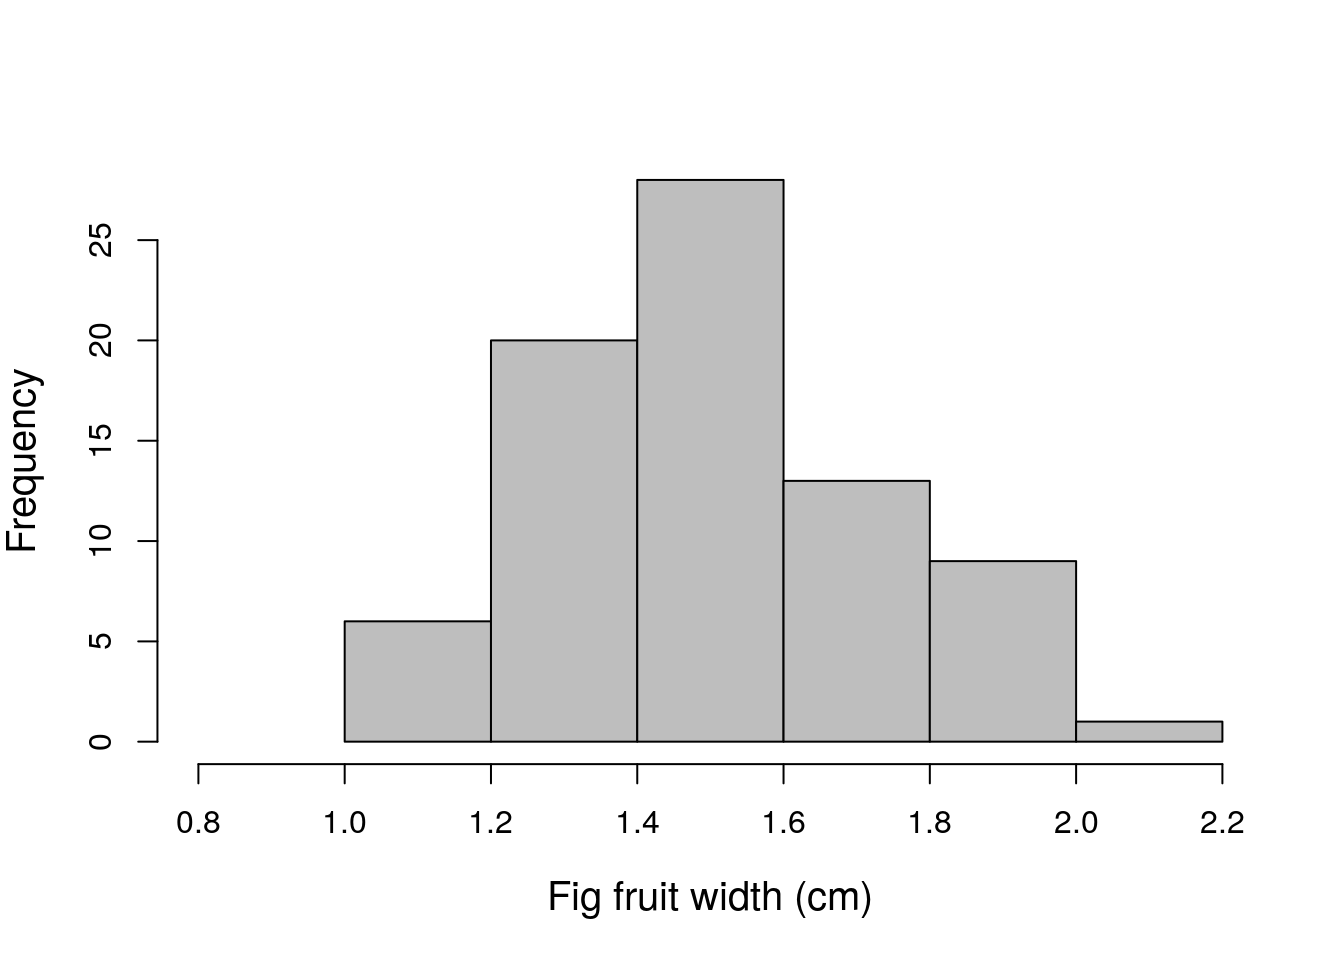
\includegraphics[width=1\linewidth]{bookdown-demo_files/figure-latex/unnamed-chunk-19-1} \caption{Boxplot of fig fruit widths (cm) collected from 4 separate trees sampled in 2010 from Baja, Mexico.}\label{fig:unnamed-chunk-19}
\end{figure}

The boxplot in Figure 10.6 can be used to quickly compare the distribution of Trees A-D.
The point at the bottom of the distribution of Tree A shows an outlier.
This outlier is an especially low value of fig fruit width compared to the other fruits of Tree A.

\hypertarget{Chapter_11}{%
\chapter{Measures of central tendency}\label{Chapter_11}}

Summary statistics describe properties of data in a single number (e.g., the mean), or a set of numbers (e.g., quartiles).
This chapter focuses on summary statistics that describe the centre of a distribution.
It also introduces quantiles, which divide a distribution into different percentages of the data (e.g., the lowest 50\% or highest 75\%).
Throughout this section, verbal and mathematical explanations of summary statistics will be presented alongside histograms or boxplots that convey the same information.
The point of doing this is to help connect the two ways of summarising the data.
All of the summary statistics that follow describe calculations for a \emph{sample} and are therefore estimates of the true values in a \emph{population}.
Recall from \protect\hyperlink{Chapter_4}{Chapter 4} the difference between a population and a sample.
This module focuses on statistical techniques, not statistical theory, so summary statistics will just focus on how to estimate statistics from sampled data instead of how statistics are defined mathematically\footnote{If interested, a good textbook for learning about theoretical statistics and the mathematics underlying what we do in this module is \citet{Miller2004}. Note, \citet{Miller2004} will not be useful for this module.}.

\hypertarget{the-mean}{%
\section{The mean}\label{the-mean}}

The arithmetic mean (hereafter just \emph{the mean}\footnote{There are other types of means, such as the geometric mean or the harmonic mean, but we will not use these at all in this module.}) of a sample is one of the most commonly reported statistics when communicating information about a dataset.
The mean is a measure of central tendency, so it is located somewhere in the centre of a distribution.
Figure 10.7 shows the same histogram of fig fruit widths shown in Figure 10.1, but with an arrow indicating where the mean of the distribution is located

\begin{figure}
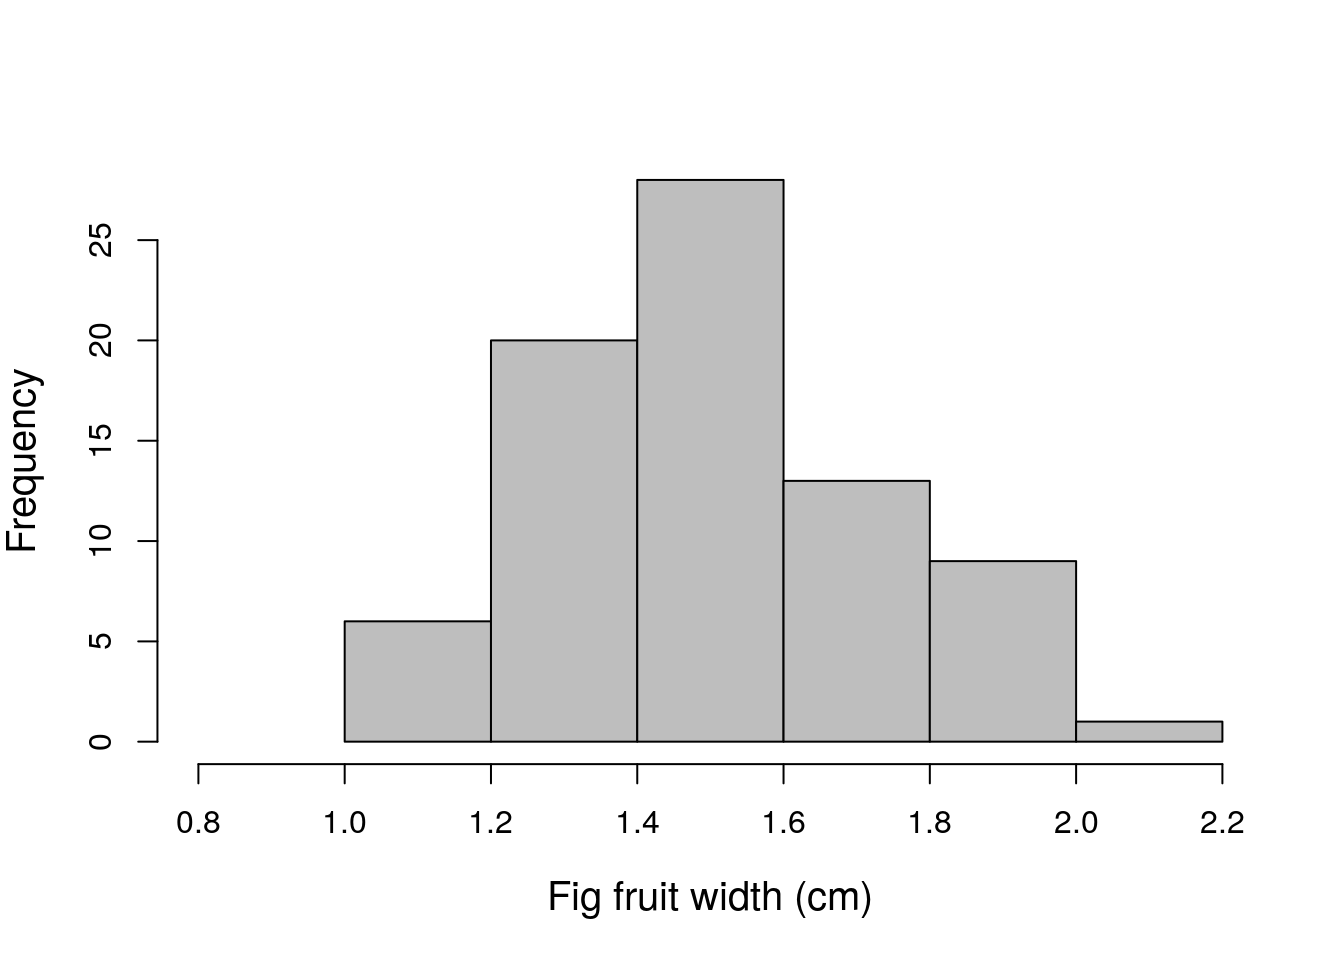
\includegraphics[width=1\linewidth]{bookdown-demo_files/figure-latex/unnamed-chunk-20-1} \caption{Example histogram fig fruit width (cm) using data from 78 fig fruits collected in in 2010 from Baja, Mexico.}\label{fig:unnamed-chunk-20}
\end{figure}

The mean is calculated by adding up the values of all of the data and dividing this sum by the total number of data \citep{Sokal1995}.
This is a fairly straightforward calculation, so we can use the mean as an example to demonstrate some new mathematical notation that will be used throughout the module.
We will start with a concrete example with actual numbers, then end with a more abstract equation describing how any sample mean is calculated.
The notation might be a bit confusing at first, but learning it will make understanding statistical concepts easier later in the module.
There are a lot of equations in what follows, but this is because we want to explain what is happening as clearly as possible, step by step.
We start with the following 8 values.

\begin{verbatim}
4.2, 5.0, 3.1, 4.2, 3.8, 4.6, 4.0, 3.5
\end{verbatim}

To calculate the mean of a sample, we just need to add up all of the values and divide by 8 (the total number of values),

\[\bar{x} = \frac{4.2 + 5.0 + 3.1 + 4.2 + 3.8 + 4.6 + 4.0 + 3.5}{8}.\]

Note that I have used the symbol \(\bar{x}\) to represent the mean of \(x\), which is a common notation \citep{Sokal1995}.
In the example above, \(\bar{x} = 4.05\).

Writing the calculation above is not a problem because we only have 8 points of data.
But sample sizes are often much larger than 8.
If we had a sample size of 80 or 800, then there is no way that we could write down every number to show how the mean is calculated.
One way to get around this is to use ellipses and just show the first and last couple of numbers,

\[\bar{x} = \frac{4.2 + 5.0 + ... + 4.0 + 3.5}{8}.\]

This is a more compact, and perfectly acceptable, way to write the sample mean.
But it is often necessary to have an even more compact way of indicating the sum over a set of values (i.e., the top of the fraction above).
To do this, each value can be symbolised by an \(x\), with a unique subscript \(i\), so that \(x_{i}\) corresponds to a specific value in the list above.
The usefulness of this notation, \(x_{i}\), will become clear soon.
It takes some getting used to, but the table below shows each symbol with its corresponding value to make it more intuitive.

\begin{longtable}[]{@{}ll@{}}
\toprule
Symbol & Value \\
\midrule
\endhead
\(x_{1}\) & 4.2 \\
\(x_{2}\) & 5.0 \\
\(x_{3}\) & 3.1 \\
\(x_{4}\) & 4.2 \\
\(x_{5}\) & 3.8 \\
\(x_{6}\) & 4.6 \\
\(x_{7}\) & 4.0 \\
\(x_{8}\) & 3.5 \\
\bottomrule
\end{longtable}

Note that we can first replace the actual values with their corresponding \(x_{i}\), so the mean can be written as,

\[\bar{x} = \frac{x_{1} + x_{2} + x_{3} + x_{4} + x_{5} + x_{6} + x_{7} + x_{8}}{8}.\]
Next, we can rewrite the top of the equation in a different form using a summation sign,

\[\sum_{i = 1}^{8}x_{i} = x_{1} + x_{2} + x_{3} + x_{4} + x_{5} + x_{6} + x_{7} + x_{8}.\]
Like the use of \(x_{i}\), the summation sign \(\sum\) takes some getting used to, but here it just means ``sum up all of the \(x_{i}\) values''.
You can think of it as a big `S' that just says ``sum up''.
The bottom of the S is the starting point and the top of it is the ending point for adding numbers.
Verbally, we can read this as saying, ``starting with \(i = 1\), add up all of the \(x_{i}\) values until \(i = 8\)''.
We can then replace the long list of \(x\) values with a summation,

\[\bar{x} = \frac{\sum_{i = 1}^{8}x_{i}}{8}.\]

This looks a bit messy, so we can rewrite the above equation.
Instead of dividing the summation by 8, we can multiply it by 1/8, which gives us the same answer,

\[\bar{x} = \frac{1}{8}\sum_{i = 1}^{8}x_{i}.\]

There is one more step.
We have started with 8 actual values and ended with a compact and abstract equation for calculating the mean.
But if we want a general description for calculating \emph{any} mean, then we need to account for sample sizes not equal to 8.
To do this, we can use \(N\) to represent the sample size.
In our example, \(N = 8\), but it is possible to have a sample size be any finite value above zero.
We can therefore replace 8 with \(N\) in the equation for the sample mean,

\[\bar{x} = \frac{1}{N}\sum_{i = 1}^{N}x_{i}.\]

There we have it.
Verbally, the above equation tells us to multiply \(1/N\) by the sum of all \(x_{i}\) values from 1 to \(N\).
This describes the mean for any sample that we might collect.

\hypertarget{the-mode}{%
\section{The mode}\label{the-mode}}

Explanation of the mode

\hypertarget{the-median-and-quantiles}{%
\section{The median and quantiles}\label{the-median-and-quantiles}}

Notes on the median and quantiles

\hypertarget{Chapter_12}{%
\chapter{Measures of spread}\label{Chapter_12}}

\hypertarget{the-range}{%
\section{The range}\label{the-range}}

\hypertarget{the-inter-quartile-range}{%
\section{The inter-quartile range}\label{the-inter-quartile-range}}

\hypertarget{the-variance}{%
\section{The variance}\label{the-variance}}

\hypertarget{the-standard-deviation}{%
\section{The standard deviation}\label{the-standard-deviation}}

\hypertarget{the-coefficient-of-variation}{%
\section{The coefficient of variation}\label{the-coefficient-of-variation}}

\hypertarget{the-standard-error}{%
\section{The standard error}\label{the-standard-error}}

\hypertarget{Chapter_13}{%
\chapter{\texorpdfstring{\emph{Practical}. Plotting and statistical summaries in Jamovi}{Practical. Plotting and statistical summaries in Jamovi}}\label{Chapter_13}}

This practical focuses on applying the concepts from Chapters 9-12 in Jamovi.
The data that we will work with in this practical were collected from a research project conducted by Dr Alan Law, Prof Nils Bunnefeld, and Prof Nigel Willby at the University of Stirling \citep{Law2014}.
The project focused on beaver reintroduction in Scottish habitats and its consequences for the white water lily, \emph{Nymphaea alba}, which beavers regularly consume (Figure 13.1)\footnote{This figure was released into the public domain by \href{https://commons.wikimedia.org/wiki/File:Nymphaea_alba._Reader.jpg}{Аlexej Potupin} on 8 June 2018.}.

\begin{figure}
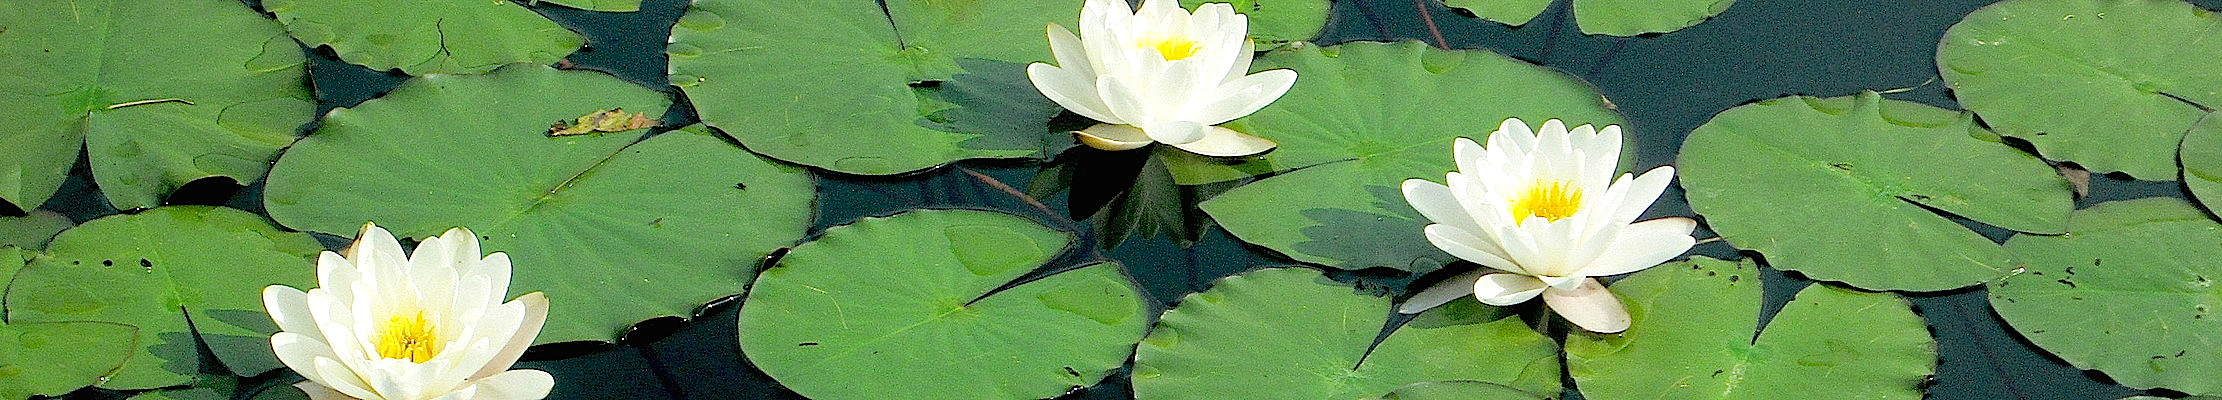
\includegraphics[width=1\linewidth]{img/Nymphaea_alba_pads} \caption{Photo of white water lillies on the water.}\label{fig:unnamed-chunk-21}
\end{figure}

As an instructive example, this lab will use the data from \citet{Law2014} on the petiole diameter (mm) from \emph{N. alba} collected from 7 different sites on the west coast of Scotland (the petiole is the structure that attaches the plant stem to the blade of the leaf).
The \emph{N. alba} dataset is available to download \href{https://raw.githubusercontent.com/bradduthie/statistical_techniques/main/data/Nymphaea_alba.csv}{here}.
Note that the data are not in a tidy format, so it is important to first reorganise the data so that they can be analysed in Jamovi (13.1).
Once the data are properly organised, we will use Jamovi to plot them (13.2), calculate summary statistics (13.3), apply appropriate decimals, significant figures, and rounding (13.4), and compare petiole diameters across sites (13.5).

\hypertarget{reorganise-the-dataset-into-a-tidy-format}{%
\section{Reorganise the dataset into a tidy format}\label{reorganise-the-dataset-into-a-tidy-format}}

The \emph{N. alba} dataset is not in a tidy format.
All of the numbers from this dataset are measurements of petiole diameter in mm from \emph{N. alba}, but each row contains 7 samples because each column shows a different site.
The full dataset is shown below.

\begin{verbatim}
##    Lily_Loch Choille.Bharr Creig.Moire Fidhle Buic Linne Beag
## 1       7.42          2.39        2.39   2.97 2.84  3.73 6.12
## 2       3.58          4.22        4.65   6.68 4.19  5.21 3.23
## 3       7.47          2.41        5.16   3.78 6.50  3.78 7.04
## 4       6.07          5.54        2.87   7.11 3.20  3.71 3.05
## 5       6.81          3.56        6.63   2.74 4.14  6.93 7.06
## 6       8.05          5.72        7.42   4.75 2.51  6.40 9.58
## 7       7.24          4.72        3.66   5.59 8.53  1.57 4.62
## 8       7.90          5.05        7.26   3.94 6.25  3.20 8.66
## 9       6.15          6.76        3.71   5.44 6.17  4.55 3.96
## 10      6.20          5.64        3.20   4.98 3.53  2.62 5.26
## 11      7.26          4.06        5.99   4.24 5.03  3.48 3.53
## 12      7.06          9.25        6.38   5.51 6.10  2.67 8.33
## 13      6.45          5.99        5.49   6.48 4.98  9.40 5.41
## 14      3.66          4.57        4.93   5.69 5.21  6.86 7.32
## 15      4.37          6.96        7.29   2.79 5.03  6.20 5.46
## 16      4.55          6.78        6.10   5.72 7.19  4.93 4.34
## 17      3.81          7.29        5.97   4.39 6.32  5.18 6.35
## 18      2.77          5.16        9.93   7.19 7.04  6.12 6.12
## 19      1.91          8.64        8.28   7.29 6.35  7.26 5.11
## 20      2.62          7.01        7.24   8.18 6.30  9.14 8.18
\end{verbatim}

Remember that to make these data tidy and usable in Jamovi, we need each row to be an independent sample.
What we really want then is a dataset with two columns of data.
The first column should indicate the site, and the second column should indicate the petiole diameter.
This can be done in two ways.
First, we could use a spreadsheet programme like LibreOffice or MS Excel to create a new dataset with two columns, one column with the site information and the other column with the petiole diameters.
Second, we could use the `Data' tab in Jamovi to create two new columns of data (one for site and the other for petiole diameter).
Either way, we need to copy and paste site names into the first column and petiole diameters in the second column.
This is a bit tedious, and we will not ask you to do it for every dataset, but it is an important step in the process of data analysis.
See Figure 13.2 for how this would look in Jamovi.

\begin{figure}
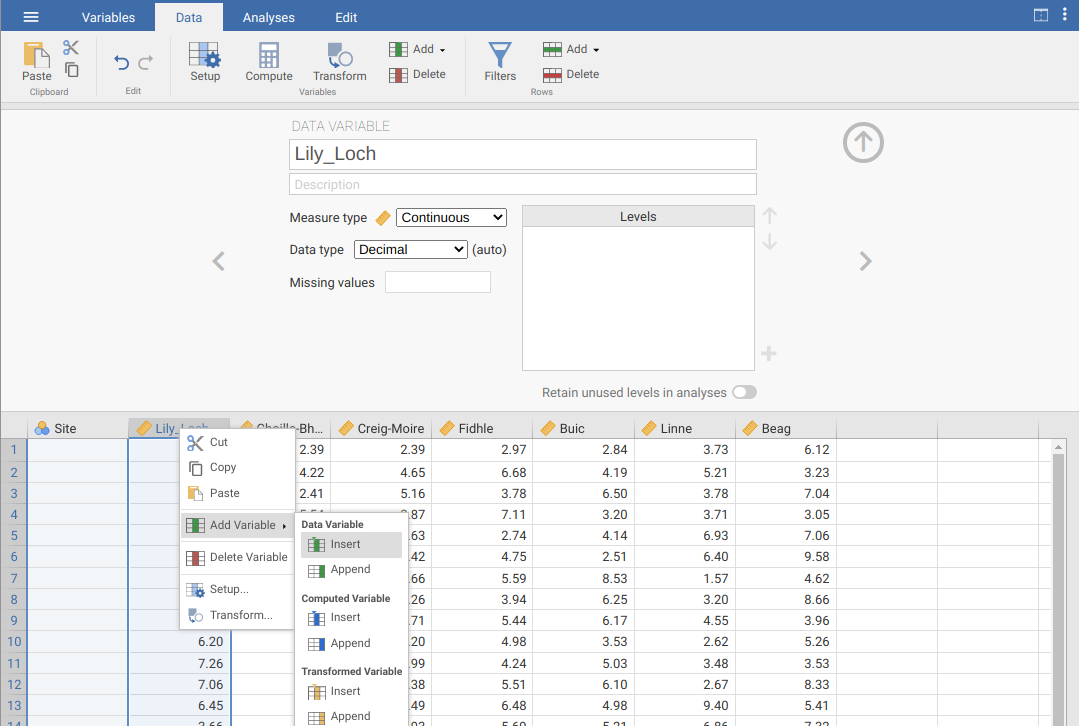
\includegraphics[width=1\linewidth]{img/lilypad_tidy} \caption{Tidying the raw data of petiole diameters from lily pad measurements across 7 sites in Scotland. A new column of data is created by right clicking on an existing column and choosing 'Add Variable'.}\label{fig:unnamed-chunk-23}
\end{figure}

Note that to insert a new column, we need to right click on an existing column and select `Add Variable' \(\to\) `Insert'.
A new column will then pop up in Jamovi, and we can give this an informative name.
Make sure to specify that the `Site' column should be a nominal measure type, and the `petiole\_diameter\_mm' column should be a continuous measure type.
The first 6 rows of the dataset should look like the below.

\begin{verbatim}
##        Site petiole_diameter_mm
## 1 Lily_Loch                7.42
## 2 Lily_Loch                3.58
## 3 Lily_Loch                7.47
## 4 Lily_Loch                6.07
## 5 Lily_Loch                6.81
## 6 Lily_Loch                8.05
\end{verbatim}

With the reorganised dataset, we are now ready to do some analysis in Jamovi.
We will start with some plotting.

\hypertarget{histograms-and-box-whisker-plots}{%
\section{Histograms and box-whisker plots}\label{histograms-and-box-whisker-plots}}

We will start by making a histogram of the full dataset of petiole diameter.
To do this, we need to go to `Analyses' tab of the Jamovi toolbar, then select the `Exploration' button.

\begin{figure}
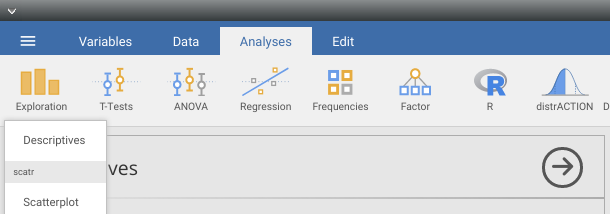
\includegraphics[width=1\linewidth]{img/lilypad_descriptives} \caption{Jamovi toolbar after having selected on the Analyses tab followed by the Exploration button.}\label{fig:unnamed-chunk-25}
\end{figure}

Next, select the `Descriptives' option (Figure 13.3).
This will open a new window where it is possible to create plots and calculate summary statistics.
The white box on the left of the Descriptive interface lists all of the variables in the dataset.
Below this box, there are options for selecting different summary statistics `Statistics' and building different graphs `Plots'.
To get started, select the petiole diameter variable in the box to the left, then move it to the `Variables' box (top right) using the \(\to\) arrow.
Next, open the Plots option at the bottom of the interface.
Choose the `Histogram' option by clicking the checkbox.
A histogram will open up in the window on the right (you might need to scroll down).

\begin{figure}
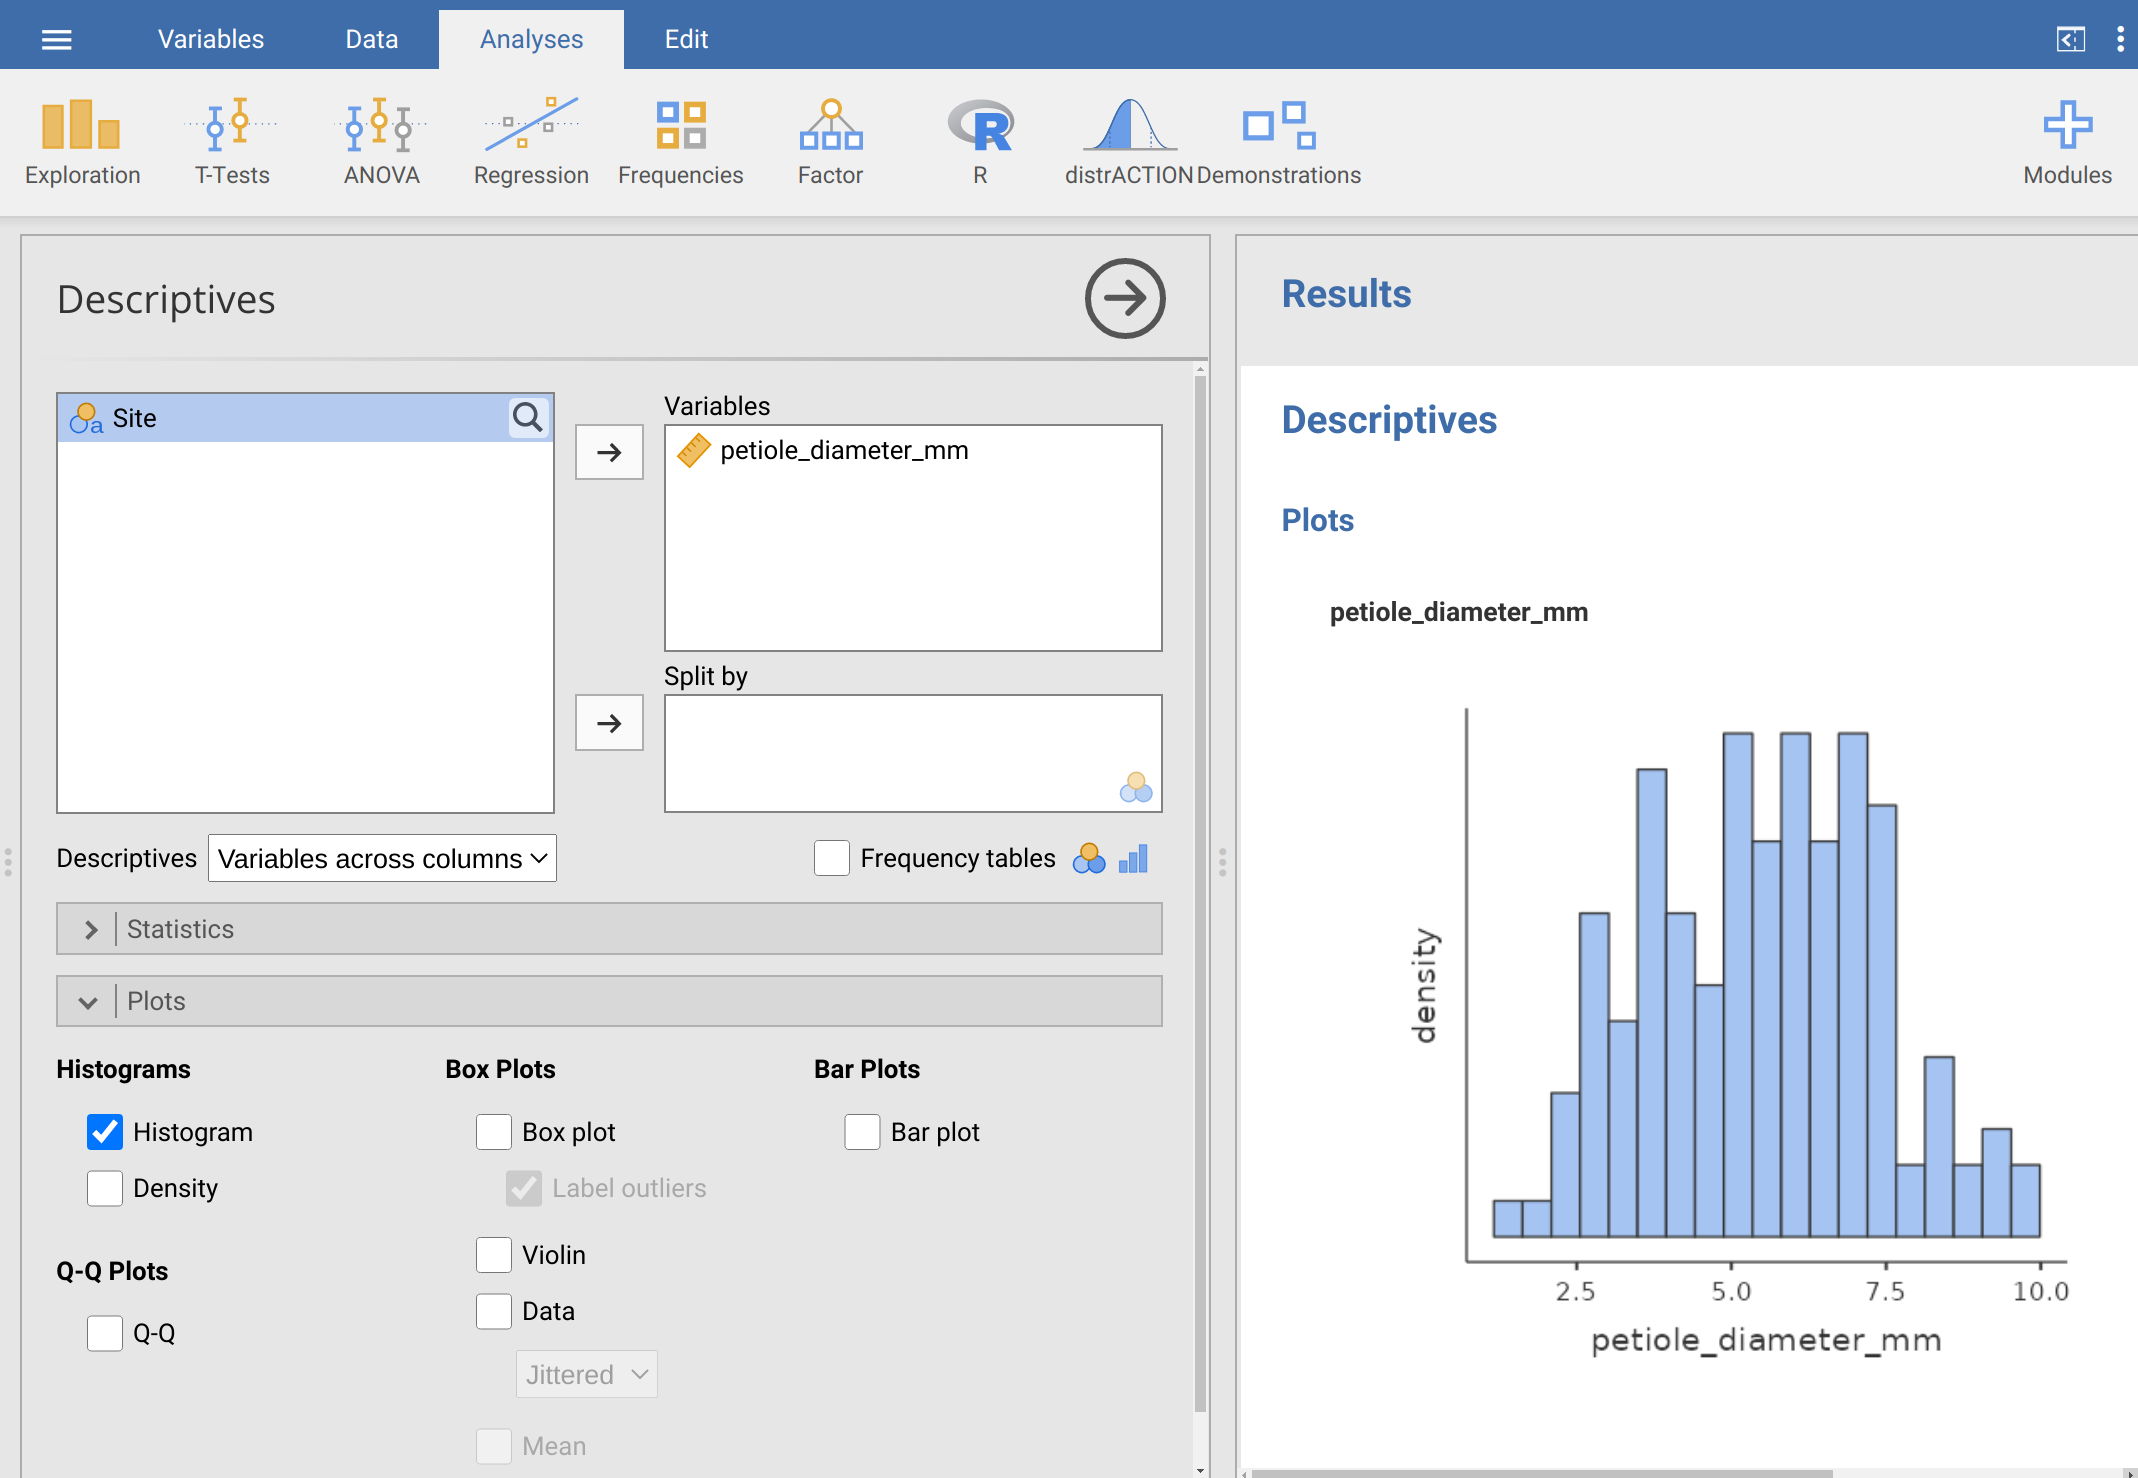
\includegraphics[width=1\linewidth]{img/lilypad_histogram} \caption{Jamovi Descriptives toolbar with petiole diameter selected and a histogram produced in the plotting window.}\label{fig:unnamed-chunk-26}
\end{figure}

Take a look at the histogram to the right (Figure 13.4).
Just looking at the histogram, write down what you think the following summary statistics will be.

Mean: \_\_\_\_\_\_\_\_\_\_\_\_\_\_\_\_\_\_\_\_\_\_\_\_\_\_\_\_

Median: \_\_\_\_\_\_\_\_\_\_\_\_\_\_\_\_\_\_\_\_\_\_\_\_\_\_\_\_

Standard deviation: \_\_\_\_\_\_\_\_\_\_\_\_\_\_\_\_\_\_\_\_\_\_\_\_\_\_\_\_

Based on the histogram, do you think that the mean and median are the same? Why or why not?

\begin{verbatim}






\end{verbatim}

The histogram needs an informative caption.
To write one in Jamovi, click on the `Edit' tab at the very top of the toolbar.
You will see some blue boxes above and below the histogram, and you can write your caption by clicking on the box immediately below the histogram.
Write a caption for the histogram below.

\begin{verbatim}






\end{verbatim}

If you want to save the histogram, then you can right click on it.
A pop-up box will give you several options; select `Image \(\to\) Export' to save the histogram.
You can save it as a PDF, PNG, SVG, or EPS (if in doubt, PNG is probably the easiest to use).
You do not need to do this for this lab, but knowing how to do it will be useful for other modules, including your fourth year dissertation.

In the first example, we looked at petiole diameters across the entire dataset, but suppose that we want to see how the data are distributed for each site individually.
To do this, we just need to go back to the Descriptives box (Figure 13.4) and put the `Site' variable into the box on the lower right called `Split by'.
Do this by selecting `Site' then using the lower \(\to\) arrow to bring it to the `Split by' box.
Instead of one histogram of petiole diameters, you will now see 7 different histograms, one for each site, all stacked on top of each other.
This might be useful, but all of these histograms together are a bit busy.
Instead, we can use a box-whisker plot to compare the distributions of petiole diameters across different sites.

To create a box plot, simply check `Box plot' from the Plots options (you might want to uncheck `Histogram', but it is not necessary).
You should now see all of the different sites on the x-axis of the newly created boxplot and a summary of the petiole diameters on the y-axis.
Based on the boxplot, which site appears to have the highest and lowest median petiole diameter?

Highest: \_\_\_\_\_\_\_\_\_\_\_\_\_\_\_\_\_\_\_\_\_\_\_\_\_\_\_\_

Lowest: \_\_\_\_\_\_\_\_\_\_\_\_\_\_\_\_\_\_\_\_\_\_\_\_\_\_\_\_

There is one more trick with box-whisker plots in Jamovi that is useful.
The current plots show a summary of each site, but it might also be useful to plot the actual data points to give some more information about the distribution of petiole diameters.
You can do this by checking the option `Data', which places the petiole diameter of each sample over the box and whiskers for each site.
The y-axis shows the petiole diameter of each data point.
By default, the points are jittered on the x-axis, which just means that they are placed randomly on the x-axis within a site.
This is just to ensure that points will not be placed directly on top of each other if they are the same value.
If you prefer, you can use the pull-down menu right below the Data checkbox to select `Stacked' instead of `Jittered'
The stacked option will place points side by side.
Think about where the points are in relation to the box and whiskers of the plot; this should help you develop an intuitive understanding of how to read box-whisker plots.

\hypertarget{calculate-summary-statistics}{%
\section{Calculate summary statistics}\label{calculate-summary-statistics}}

We can calculate the summary statistics using the `Descriptives' option in Jamovi, just as we did with the histogram and box-whisker plots.
Before doing anything else, again place the petiole diameter variable in the box of variables, but do not split the dataset by site just yet because we first want summary statistics across the entire dataset.
Below the box of variables, but above the Plots options, there are options for selecting different summary statistics.
Open up this new box and have a look at the different summary statistics that can be calculated.
To calculate all of the variables explained in \protect\hyperlink{Chapter_11}{Chapter 11} and \protect\hyperlink{Chapter_11}{Chapter 12}, check the following 11 boxes:

\begin{itemize}
\tightlist
\item
  N: \_\_\_\_\_\_\_\_\_\_\_\_\_\_\_\_\_\_\_\_\_\_\_
\item
  Std. deviation: \_\_\_\_\_\_\_\_\_\_\_\_\_\_\_\_\_\_\_\_\_\_\_
\item
  Variance: \_\_\_\_\_\_\_\_\_\_\_\_\_\_\_\_\_\_\_\_\_\_\_
\item
  Range: \_\_\_\_\_\_\_\_\_\_\_\_\_\_\_\_\_\_\_\_\_\_\_
\item
  Minimum: \_\_\_\_\_\_\_\_\_\_\_\_\_\_\_\_\_\_\_\_\_\_\_
\item
  Maximum: \_\_\_\_\_\_\_\_\_\_\_\_\_\_\_\_\_\_\_\_\_\_\_
\item
  Range: \_\_\_\_\_\_\_\_\_\_\_\_\_\_\_\_\_\_\_\_\_\_\_
\item
  IQR: \_\_\_\_\_\_\_\_\_\_\_\_\_\_\_\_\_\_\_\_\_\_\_
\item
  Mean: \_\_\_\_\_\_\_\_\_\_\_\_\_\_\_\_\_\_\_\_\_\_\_
\item
  Median: \_\_\_\_\_\_\_\_\_\_\_\_\_\_\_\_\_\_\_\_\_\_\_
\item
  Mode: \_\_\_\_\_\_\_\_\_\_\_\_\_\_\_\_\_\_\_\_\_\_\_
\item
  Std. error of mean: \_\_\_\_\_\_\_\_\_\_\_\_\_\_\_\_\_\_\_\_\_\_\_
\end{itemize}

When you do this, the Statistics option in Jamovi should like like it does in Figure 13.5.

\begin{figure}
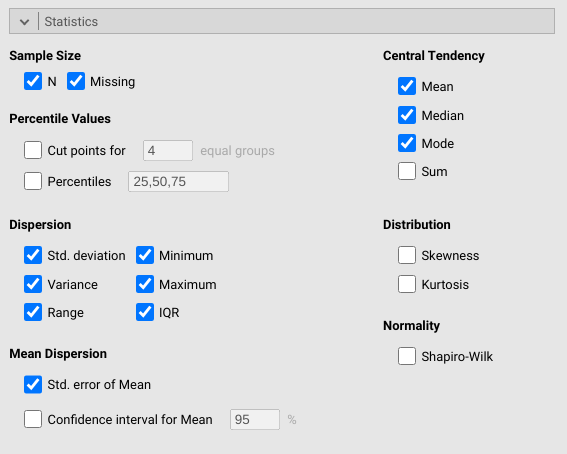
\includegraphics[width=1\linewidth]{img/lilypad_summary_statistics} \caption{Jamovi Descriptives toolbar showing the summary statistics available to report.}\label{fig:unnamed-chunk-27}
\end{figure}

Once you check these boxes, you will see a `Descriptives' table open on the right hand side of Jamovi.
This table will report all of the summary statistics that you have checked.
Write down the values for the summary statistics next to the corresponding bullet points above.

Next split these summary statistics up by site.
Notice the very large table that is now produced on the right hand side of Jamovi.
Which of the 7 sites in the data set has the highest mean petiole diameter, and what is its mean?

Site: \_\_\_\_\_\_\_\_\_\_\_\_\_\_\_\_\_\_\_\_\_\_\_\_\_\_\_\_\_\_

Mean: \_\_\_\_\_\_\_\_\_\_\_\_\_\_\_\_\_\_\_\_\_\_\_\_\_\_\_\_\_\_

Which of the 7 sites has the lowest variation in petiole diameter, and what is its variation?

Site: \_\_\_\_\_\_\_\_\_\_\_\_\_\_\_\_\_\_\_\_\_\_\_\_\_\_\_\_\_\_

Variation: \_\_\_\_\_\_\_\_\_\_\_\_\_\_\_\_\_\_\_\_\_\_\_\_\_\_\_\_\_\_

Make sure that you are able to find and interpret these summary statistics in Jamovi.
Explore different options to get more comfortable using Jamovi for building plots and reporting summary statistics.
Can you find the first and third quartiles for each site?
Report the third quartiles for each site below.

Beag: \_\_\_\_\_\_\_\_\_\_\_\_\_\_\_\_\_\_\_\_\_\_\_\_\_\_\_\_\_\_

Buic: \_\_\_\_\_\_\_\_\_\_\_\_\_\_\_\_\_\_\_\_\_\_\_\_\_\_\_\_\_\_

Choille-Bharr: \_\_\_\_\_\_\_\_\_\_\_\_\_\_\_\_\_\_\_\_\_\_\_\_\_\_\_\_\_\_

Creig-Moire: \_\_\_\_\_\_\_\_\_\_\_\_\_\_\_\_\_\_\_\_\_\_\_\_\_\_\_\_\_\_

Fidhle: \_\_\_\_\_\_\_\_\_\_\_\_\_\_\_\_\_\_\_\_\_\_\_\_\_\_\_\_\_\_

Lily\_Loch: \_\_\_\_\_\_\_\_\_\_\_\_\_\_\_\_\_\_\_\_\_\_\_\_\_\_\_\_\_\_

Linne: \_\_\_\_\_\_\_\_\_\_\_\_\_\_\_\_\_\_\_\_\_\_\_\_\_\_\_\_\_\_

Next, we will look at reporting summary statistics to different significant figures.

\hypertarget{reporting-decimals-and-significant-figures}{%
\section{Reporting decimals and significant figures}\label{reporting-decimals-and-significant-figures}}

Using the same values that you reported above for the whole dataset (i.e., not broken down by site), report each summary statistics to two significant figures.
Remember to round accurately if you need to reduce the number of significant figures from the original values to the new values below.
In assessments, you will often be asked to report a particular answer to a specific number of decimal places or significant figures, so the intention here is to help you practice.

\begin{itemize}
\tightlist
\item
  N: \_\_\_\_\_\_\_\_\_\_\_\_\_\_\_\_\_\_\_\_\_\_\_
\item
  Std. deviation: \_\_\_\_\_\_\_\_\_\_\_\_\_\_\_\_\_\_\_\_\_\_\_
\item
  Variance: \_\_\_\_\_\_\_\_\_\_\_\_\_\_\_\_\_\_\_\_\_\_\_
\item
  Range: \_\_\_\_\_\_\_\_\_\_\_\_\_\_\_\_\_\_\_\_\_\_\_
\item
  Minimum: \_\_\_\_\_\_\_\_\_\_\_\_\_\_\_\_\_\_\_\_\_\_\_
\item
  Maximum: \_\_\_\_\_\_\_\_\_\_\_\_\_\_\_\_\_\_\_\_\_\_\_
\item
  Range: \_\_\_\_\_\_\_\_\_\_\_\_\_\_\_\_\_\_\_\_\_\_\_
\item
  IQR: \_\_\_\_\_\_\_\_\_\_\_\_\_\_\_\_\_\_\_\_\_\_\_
\item
  Mean: \_\_\_\_\_\_\_\_\_\_\_\_\_\_\_\_\_\_\_\_\_\_\_
\item
  Median: \_\_\_\_\_\_\_\_\_\_\_\_\_\_\_\_\_\_\_\_\_\_\_
\item
  Mode: \_\_\_\_\_\_\_\_\_\_\_\_\_\_\_\_\_\_\_\_\_\_\_
\item
  Std. error of mean: \_\_\_\_\_\_\_\_\_\_\_\_\_\_\_\_\_\_\_\_\_\_\_
\end{itemize}

Remember from 13.2 that you were asked to write down what you thought the mean, median, and standard deviation were just by inspecting the histogram.
Compare your answers in that section with the rounded statistics listed above.
Were you able to get a similar value from the histogram as calculated in Jamovi from the data?
What can you learn from the histogram that you cannot from the summary statistics, and what can you learn from the summary statistics that you cannot from the histogram?
Write your reflections in the space below.

\begin{verbatim}






\end{verbatim}

Next, we will produce barplots to show the mean petiol diameter for each site.

\hypertarget{comparing-across-sites}{%
\section{Comparing across sites}\label{comparing-across-sites}}

To make a barplot that compares the mean petiole diameters across sites, we again use the Descriptives option in Jamovi.
Place petiole diameter as the variable, and spit this by site.
Next, go down to the plotting options and check `Bar plot'.
You will see a barplot produced in the window to the right with different sites on the x-axis.
Bar heights show the mean petiole diameter for each site.
Notice the intervals shown for each bar (i.e., the vertical lines in the centre of the bars that go up and down different lengths).
These error bars are centred on the mean petiole diameter (bar height) and show one standard error above and below the site mean.
Recall back from \protect\hyperlink{Chapter_12}{Chapter 12}; what information do these error bars convey about the estimated mean petiole diameter?

\begin{verbatim}






\end{verbatim}

What can you say about the mean petiole diameters across the different sites?
Do these sites appear to have very different mean petiole diameters?

\begin{verbatim}






\end{verbatim}

There were 20 total petiole diameters sampled from each site.
If we were to go back out to these 7 sites and sample another 20 petiole diameters, could we \textbf{really} expect to get the exact same site means?
Assuming the site means would be at least a bit different for our new sample, is it possible that the sites with the highest or lowest petiole diameters might also be different in our new sample?
If so, then what does this say about our ability to make conclusions about the differences in petiole diameter among sites?

\begin{verbatim}






\end{verbatim}

\hypertarget{part-probability-models-and-the-central-limit-theorem}{%
\part{Probability models and the Central Limit Theorem}\label{part-probability-models-and-the-central-limit-theorem}}

\hypertarget{week-4-overview}{%
\chapter*{Week 4 Overview}\label{week-4-overview}}
\addcontentsline{toc}{chapter}{Week 4 Overview}

General overview of what will be the focus of this week.

Week: 4
Dates:
Suggested Readings: Textbook intro to probability
Assessments: Practice quiz
Practical:

\hypertarget{introduction-to-probability-models}{%
\chapter{Introduction to probability models}\label{introduction-to-probability-models}}

Some background

\hypertarget{a-practical-example}{%
\section{A practical example}\label{a-practical-example}}

How to think about probability

\hypertarget{probability-distributions}{%
\section{Probability distributions}\label{probability-distributions}}

Some more useful examples

\hypertarget{binomial-distribution}{%
\subsection{Binomial distribution}\label{binomial-distribution}}

Explanation, fairly straightforward

\hypertarget{poisson-distribution}{%
\subsection{Poisson distribution}\label{poisson-distribution}}

Another example

\hypertarget{normal-distribution}{%
\subsection{Normal distribution}\label{normal-distribution}}

Why this is so important

\hypertarget{the-central-limit-theorem-clt}{%
\chapter{The Central Limit Theorem (CLT)}\label{the-central-limit-theorem-clt}}

General overview

\hypertarget{examples-of-the-clt-in-action}{%
\section{Examples of the CLT in action}\label{examples-of-the-clt-in-action}}

\hypertarget{the-standard-normal-distribution}{%
\section{The standard normal distribution}\label{the-standard-normal-distribution}}

\hypertarget{what-are-z-scores}{%
\section{What are z-scores?}\label{what-are-z-scores}}

\hypertarget{practical.-probability-and-simulation}{%
\chapter{\texorpdfstring{\emph{Practical}. Probability and simulation}{Practical. Probability and simulation}}\label{practical.-probability-and-simulation}}

Some of these examples will be similar to what will be on the assessment

\hypertarget{calculating-probability-exercise-1}{%
\section{Calculating probability exercise 1}\label{calculating-probability-exercise-1}}

Example exercise 1 with some simple probability calculations

\hypertarget{calculating-probability-exercise-2}{%
\section{Calculating probability exercise 2}\label{calculating-probability-exercise-2}}

Example exercise 2 with some simple probability calculations

\hypertarget{calculating-probability-from-normal-distribution}{%
\section{Calculating probability from normal distribution}\label{calculating-probability-from-normal-distribution}}

Example exercise for getting a the probability of some value sampled above, below, or between some threshold in Jamovi.

\hypertarget{normal-distribution-and-sample-size}{%
\section{Normal distribution and sample size}\label{normal-distribution-and-sample-size}}

Showing how we get closer to the normal distribution as sample size increases in Jamovi.

\hypertarget{simulating-the-central-limit-theorem}{%
\section{Simulating the central limit theorem}\label{simulating-the-central-limit-theorem}}

Doing the example from a uniform distribution in Jamovi.

\hypertarget{part-statistical-inference}{%
\part{Statistical inference}\label{part-statistical-inference}}

\hypertarget{week-5-overview}{%
\chapter*{Week 5 Overview}\label{week-5-overview}}
\addcontentsline{toc}{chapter}{Week 5 Overview}

General overview of what will be the focus of this week.

Week: 5
Dates:
Suggested Readings: Textbook intro to probability
Assessments: Practice quiz
Practical:

\hypertarget{sample-statistics-and-population-parameters}{%
\chapter{Sample statistics and population parameters}\label{sample-statistics-and-population-parameters}}

An explanation of this

\hypertarget{standard-normal-distribution}{%
\chapter{Standard Normal Distribution}\label{standard-normal-distribution}}

What this means, and why it is important.

\hypertarget{confidence-intervals}{%
\chapter{Confidence intervals}\label{confidence-intervals}}

How these are calculated, and how to interpret them

\hypertarget{the-t-interval}{%
\chapter{The t-interval}\label{the-t-interval}}

What this is and how it relates to the normal distribution, and why it is important.

\hypertarget{practical.-z--and-t--intervals}{%
\chapter{\texorpdfstring{\emph{Practical}. z- and t- intervals}{Practical. z- and t- intervals}}\label{practical.-z--and-t--intervals}}

\hypertarget{example-constructing-confidence-intervals}{%
\section{Example constructing confidence intervals}\label{example-constructing-confidence-intervals}}

\hypertarget{confidence-interval-for-different-levels-t--and-z-}{%
\section{Confidence interval for different levels (t- and z-)}\label{confidence-interval-for-different-levels-t--and-z-}}

\hypertarget{proportion-confidence-intervals}{%
\section{Proportion confidence intervals}\label{proportion-confidence-intervals}}

\hypertarget{another-confidence-interval-example}{%
\section{Another confidence interval example?}\label{another-confidence-interval-example}}

\hypertarget{part-review-of-parts-i-v}{%
\part{Review of parts I-V}\label{part-review-of-parts-i-v}}

\hypertarget{week-6-overview-reading-week}{%
\chapter*{Week 6 Overview (Reading week)}\label{week-6-overview-reading-week}}
\addcontentsline{toc}{chapter}{Week 6 Overview (Reading week)}

This is a special chapter for week 6, which is a reading week, and it will function as a very brief pause for review. It will also ensure that the numbers of chapters will correspond to weeks.

\hypertarget{part-hypothesis-testing}{%
\part{Hypothesis testing}\label{part-hypothesis-testing}}

\hypertarget{week-7-overview}{%
\chapter*{Week 7 Overview}\label{week-7-overview}}
\addcontentsline{toc}{chapter}{Week 7 Overview}

General overview of what will be the focus of this week.

Week: 7
Dates:
Suggested Readings: Textbook
Assessments: Practice quiz
Practical:

\hypertarget{what-is-hypothesis-testing}{%
\chapter{What is hypothesis testing?}\label{what-is-hypothesis-testing}}

An explanation of this, and that we are starting to get into some of the more interesting bits of inferential statistics.

\hypertarget{making-and-using-hypotheses-and-types-of-tests}{%
\chapter{Making and using hypotheses and types of tests}\label{making-and-using-hypotheses-and-types-of-tests}}

What this means, and why it is important.

\hypertarget{an-example-of-hypothesis-testing}{%
\chapter{An example of hypothesis testing}\label{an-example-of-hypothesis-testing}}

Errors

\hypertarget{hypothesis-testing-and-confidence-intervals}{%
\chapter{Hypothesis testing and confidence intervals}\label{hypothesis-testing-and-confidence-intervals}}

Relationship between these two.

\hypertarget{student-t-distribution-and-one-sample-t-test}{%
\chapter{Student t-distribution and one sample t-test}\label{student-t-distribution-and-one-sample-t-test}}

What this is and how to do it in Jamovi.

\hypertarget{another-example-of-a-one-sample-t-test}{%
\chapter{Another example of a one sample t-test}\label{another-example-of-a-one-sample-t-test}}

From the lectures

\hypertarget{independent-t-test}{%
\chapter{Independent t-test}\label{independent-t-test}}

What this is and how to use it in Jamovi.

\hypertarget{paired-sample-t-test}{%
\chapter{Paired sample t-test}\label{paired-sample-t-test}}

Another explanation, example, and how to do it in Jamovi.

\hypertarget{violations-of-assumptions}{%
\chapter{Violations of assumptions}\label{violations-of-assumptions}}

What to do in this case

\hypertarget{non-parametric-tests-and-what-these-are.}{%
\chapter{Non-parametric tests, and what these are.}\label{non-parametric-tests-and-what-these-are.}}

Explanation of how to do them in Jamovi.

\hypertarget{practical.-hypothesis-testing-and-t-tests}{%
\chapter{\texorpdfstring{\emph{Practical}. Hypothesis testing and t-tests}{Practical. Hypothesis testing and t-tests}}\label{practical.-hypothesis-testing-and-t-tests}}

\hypertarget{exercise-on-a-simple-one-sample-t-test}{%
\section{Exercise on a simple one sample t-test}\label{exercise-on-a-simple-one-sample-t-test}}

\hypertarget{exercise-on-an-independent-sample-t-test}{%
\section{Exercise on an independent sample t-test}\label{exercise-on-an-independent-sample-t-test}}

\hypertarget{exercise-involving-multiple-comparisons}{%
\section{Exercise involving multiple comparisons}\label{exercise-involving-multiple-comparisons}}

\hypertarget{exercise-with-non-parametric}{%
\section{Exercise with non-parametric}\label{exercise-with-non-parametric}}

\hypertarget{another-exercise-with-non-parametric}{%
\section{Another exercise with non-parametric}\label{another-exercise-with-non-parametric}}

\hypertarget{part-analysis-of-variance-anova}{%
\part{Analysis of Variance (ANOVA)}\label{part-analysis-of-variance-anova}}

\hypertarget{week-8-overview}{%
\chapter*{Week 8 Overview}\label{week-8-overview}}
\addcontentsline{toc}{chapter}{Week 8 Overview}

General overview of what will be the focus of this week.

Week: 8
Dates:
Suggested Readings: Textbook
Assessments: Practice quiz
Practical:

\hypertarget{what-is-anova}{%
\chapter{What is ANOVA?}\label{what-is-anova}}

General explanation

\hypertarget{one-way-anova}{%
\chapter{One-way ANOVA}\label{one-way-anova}}

Explain what this is.

\hypertarget{two-way-anova}{%
\chapter{Two-way ANOVA}\label{two-way-anova}}

More explanation

\hypertarget{kruskall-wallis-h-test}{%
\chapter{Kruskall-Wallis H test}\label{kruskall-wallis-h-test}}

Non-parametric explanation

\hypertarget{practical.-anova-and-associated-tests}{%
\chapter{\texorpdfstring{\emph{Practical}. ANOVA and associated tests}{Practical. ANOVA and associated tests}}\label{practical.-anova-and-associated-tests}}

\hypertarget{anova-exercise-1}{%
\section{ANOVA Exercise 1}\label{anova-exercise-1}}

\hypertarget{anova-exercise-2}{%
\section{ANOVA Exercise 2}\label{anova-exercise-2}}

\hypertarget{anova-exercise-3}{%
\section{ANOVA Exercise 3}\label{anova-exercise-3}}

\hypertarget{anova-exercise-4}{%
\section{ANOVA Exercise 4}\label{anova-exercise-4}}

\hypertarget{part-counts-and-correlation}{%
\part{Counts and Correlation}\label{part-counts-and-correlation}}

\hypertarget{week-9-overview}{%
\chapter*{Week 9 Overview}\label{week-9-overview}}
\addcontentsline{toc}{chapter}{Week 9 Overview}

General overview of what will be the focus of this week.

Week: 9
Dates:
Suggested Readings: Textbook
Assessments: Practice quiz
Practical:

\hypertarget{frequency-and-count-data}{%
\chapter{Frequency and count data}\label{frequency-and-count-data}}

General explanation

\hypertarget{chi-squared-goodness-of-fit}{%
\chapter{Chi-squared goodness of fit}\label{chi-squared-goodness-of-fit}}

Explain what this is.

\hypertarget{chi-squared-test-of-association}{%
\chapter{Chi-squared test of association}\label{chi-squared-test-of-association}}

More explanation

\hypertarget{correlation-key-concepts}{%
\chapter{Correlation key concepts}\label{correlation-key-concepts}}

\hypertarget{correlation-mathematics}{%
\chapter{Correlation mathematics}\label{correlation-mathematics}}

\hypertarget{correlation-hypothesis-testing}{%
\chapter{Correlation hypothesis testing}\label{correlation-hypothesis-testing}}

\hypertarget{practical.-analysis-of-count-data-correlation-and-regression}{%
\chapter{\texorpdfstring{\emph{Practical}. Analysis of count data, correlation, and regression}{Practical. Analysis of count data, correlation, and regression}}\label{practical.-analysis-of-count-data-correlation-and-regression}}

\hypertarget{chi-square-exercise-1}{%
\section{Chi-Square Exercise 1}\label{chi-square-exercise-1}}

\hypertarget{chi-square-association-exercise-2}{%
\section{Chi-Square association Exercise 2}\label{chi-square-association-exercise-2}}

\hypertarget{correlation-exercise-3}{%
\section{Correlation Exercise 3}\label{correlation-exercise-3}}

\hypertarget{correlation-exercise-4}{%
\section{Correlation Exercise 4}\label{correlation-exercise-4}}

\hypertarget{part-linear-regression}{%
\part{Linear Regression}\label{part-linear-regression}}

\hypertarget{week-10-overview}{%
\chapter*{Week 10 Overview}\label{week-10-overview}}
\addcontentsline{toc}{chapter}{Week 10 Overview}

Week: 10
Dates:
Suggested Readings: Textbook
Assessments: Practice quiz
Practical:

\hypertarget{regression-key-concepts}{%
\chapter{Regression key concepts}\label{regression-key-concepts}}

\hypertarget{regression-validity}{%
\chapter{Regression validity}\label{regression-validity}}

\hypertarget{introduction-to-multiple-regression}{%
\chapter{Introduction to multiple regression}\label{introduction-to-multiple-regression}}

General explanation

\hypertarget{model-selection-maybe-remove-this}{%
\chapter{Model selection (maybe remove this?)}\label{model-selection-maybe-remove-this}}

Seriously consider moving the regression into this week. and ease the amount of material in previous weeks.

\hypertarget{practical.-using-regression}{%
\chapter{\texorpdfstring{\emph{Practical}. Using regression}{Practical. Using regression}}\label{practical.-using-regression}}

\hypertarget{regression-exercise-1}{%
\section{Regression Exercise 1}\label{regression-exercise-1}}

\hypertarget{regression-exercise-2}{%
\section{Regression Exercise 2}\label{regression-exercise-2}}

\hypertarget{regression-exercise-3}{%
\section{Regression Exercise 3}\label{regression-exercise-3}}

\hypertarget{regression-exercise-4}{%
\section{Regression Exercise 4}\label{regression-exercise-4}}

\hypertarget{part-randomisation-approaches}{%
\part{Randomisation approaches}\label{part-randomisation-approaches}}

\hypertarget{week-11-overview}{%
\chapter*{Week 11 Overview}\label{week-11-overview}}
\addcontentsline{toc}{chapter}{Week 11 Overview}

The aim of this lecture is to introduce the randomisation approach to statistical hypothesis testing. We will first introduce the general idea of what randomisation is and how it relates to the hypothesis testing that we have been doing since week five. We will then consider an instructive example in which a randomisation approach is used in place of a traditional t-test to test whether or not the mean values of two different groups are identical. We will then compare the assumptions underlying randomisation and how they differ slightly from the assumptions of traditional hypothesis testing. We will then look at how randomisation can be used to build confidence intervals and test hypotheses that would difficult to test with other approaches. In learning about randomisation approaches, we will also review some key concepts from earlier in the module. The aim is not to understand all of the nuances of randomisation, but to understand, conceptually, what is going on in the methods described below.

Week: 11
Dates:
Suggested Readings: Textbook
Assessments: Practice quiz
Practical: R starts creeping in now?

\hypertarget{introduction-to-randomisation}{%
\chapter{Introduction to randomisation}\label{introduction-to-randomisation}}

General explanation

\hypertarget{assumptions-of-randomisation}{%
\chapter{Assumptions of randomisation}\label{assumptions-of-randomisation}}

How these differ

\hypertarget{bootstrapping}{%
\chapter{Bootstrapping}\label{bootstrapping}}

What this is and why we use it.

\hypertarget{monte-carlo}{%
\chapter{Monte Carlo}\label{monte-carlo}}

\hypertarget{practical.-using-r}{%
\chapter{\texorpdfstring{\emph{Practical}. Using R}{Practical. Using R}}\label{practical.-using-r}}

\hypertarget{r-exercise-1}{%
\section{R Exercise 1}\label{r-exercise-1}}

\hypertarget{r-exercise-2}{%
\section{R Exercise 2}\label{r-exercise-2}}

\hypertarget{r-exercise-3}{%
\section{R Exercise 3}\label{r-exercise-3}}

\hypertarget{part-statistical-reporting}{%
\part{Statistical Reporting}\label{part-statistical-reporting}}

\hypertarget{week-12-overview}{%
\chapter*{Week 12 Overview}\label{week-12-overview}}
\addcontentsline{toc}{chapter}{Week 12 Overview}

Week: 12
Dates:
Suggested Readings: Textbook
Assessments: Practice quiz
Practical: R starts creeping in now?

\hypertarget{reporting-statistics}{%
\chapter{Reporting statistics}\label{reporting-statistics}}

General explanation

\hypertarget{more-introduction-to-r}{%
\chapter{More introduction to R}\label{more-introduction-to-r}}

How these differ

\hypertarget{more-getting-started-with-r}{%
\chapter{More getting started with R}\label{more-getting-started-with-r}}

Just more to do.

\hypertarget{practical.-using-r-1}{%
\chapter{\texorpdfstring{\emph{Practical}. Using R}{Practical. Using R}}\label{practical.-using-r-1}}

\hypertarget{r-exercise-1-1}{%
\section{R Exercise 1}\label{r-exercise-1-1}}

\hypertarget{r-exercise-2-1}{%
\section{R Exercise 2}\label{r-exercise-2-1}}

\hypertarget{r-exercise-3-1}{%
\section{R Exercise 3}\label{r-exercise-3-1}}

\hypertarget{part-review-of-parts-vii-xii}{%
\part{Review of parts (VII-XII)}\label{part-review-of-parts-vii-xii}}

\hypertarget{module-summary}{%
\chapter*{Module summary}\label{module-summary}}
\addcontentsline{toc}{chapter}{Module summary}

This chapter will be specifically to prepare for exam.

\hypertarget{appendix-appendix}{%
\appendix}


\hypertarget{appendixA_units}{%
\chapter{Statistical units}\label{appendixA_units}}

\hypertarget{uncertainty_derivation}{%
\chapter{Uncertainty derivation}\label{uncertainty_derivation}}

It is not necessary to be able to derive the equations for propagating error from week 2, but working through the below might be interesting, and provide a better appreciation for why these formulas make sense.
Another derivation is available in \citet{Box1978} (page 563), but this derivation is expressed in terms of variances and covariances, which is likely to be less helpful for this module.

\textbf{Propagation of error for addition and subtraction}.

For adding and subtracting error, we know that we get our variable \(Z\) by adding \(X\) and \(Y\). This is just how \(Z\) is defined. We also know that \(Z\) is going to have some error \(E_Z\), and we know that \(Z\) plus or minus its error will equal \(X\) plus or minus its error plus \(Y\) plus or minus its error,

\[(Z \pm E_Z) = (X  \pm E_X) + (Y \pm E_Y).\]

Again, this is just our starting definition, but double-check to make sure it makes sense. We can now note that we know,

\[Z =X+Y.\]

If it is not intuitive as to why, just imagine that there is no error associated with the measurement of \(X\) an \(Y\) (i.e., \(E_{X} = 0\) and \(E_{Y} = 0\)).
In this case, there cannot be any error in \(Z\). So, if we substitute \(X + Y\) for \(Z\), we have the below,

\[((X + Y) \pm E_Z) = (X  \pm E_X) + (Y \pm E_Y).\]

By the \href{https://en.wikipedia.org/wiki/Associative_property}{associative property}, we can get rid of the parenthesis for addition and subtraction, giving us the below,

\[X + Y \pm E_Z = X  \pm E_X + Y \pm E_Y.\]

Now we can subtract \(X\) and \(Y\) from both sides and see that we just have the errors of \(X\), \(Y\), and \(Z\),

\[\pm E_Z = \pm E_X \pm E_Y.\]

The plus/minus is a bother. Note, however, that for any real number \(m\), \(m^{2} = (-m)^2\). For example, if \(m = 4\), then \((4)2 = 16\) and \((-4)2 = 16\), so we can square both sides to get positive numbers and make things easier,

\[E_Z^2 = (\pm E_X \pm E_Y)^2.\]
We can expand the above,

\[E_Z^2 = E_X^2 + E_Y^2 \pm2E_X E_Y.\]

Now here is an assumption that we have not told you about elsewhere in the module.
With the formulas that we have given you, we are assuming that the errors of \(X\) and \(Y\) are independent.
To put it in more statistical terms, the covariance between the errors of \(X\) and \(Y\) is assumed to be zero.
Without going into the details (covariance will be introduced later in the module), if we assume that the covariance between these errors is zero, then we can also assume the last term of the above is zero, so we can get rid of it (i.e., \(2E_{X}E_{Y} = 0\)),

\[E_Z^2 = E_X^2 + E_Y^2.\]

If we take the square root of both sides, then we have the equation from \protect\hyperlink{Chapter_7}{Chapter 7},

\[E_Z = \sqrt{E_X^2 + E_Y^2}.\]

\textbf{Propagation of error for multiplication and division}.

Now that we have seen the logic for propagating errors in addition and subtraction, we can do the same for multiplication and division.
We can start with the same point that we are getting our new variable \(Z\) by multiplying \(X\) and \(Y\) together, \(Z = XY\). So, if both \(X\) and \(Y\) have errors, the errors will be multiplicative as below,

\[Z \pm E_Z = (X \pm E_X)(Y \pm E_Y).\]

Again, all we are doing here is substituting \(Z\), \(X\), and \(Y\), for an expression in parentheses that includes the variable plus or minus its associated error.
Now we can expand the right hand side of the equation,

\[Z \pm E_Z = XY + Y E_X + X E_Y + E_X E_Y.\]

As with our propagation of error in addition, here we are also going to assume that the sources of error for \(X\) and \(Y\) are independent (i.e., their covariance is zero).
This allows us to set \(E_{X}E_{Y} = 0\), which leaves us with the below,

\[Z \pm E_Z = XY + Y E_X + X E_Y.\]

Now, because \(Z = XY\), we can substitute on the left hand side of the equation,

\[XY \pm E_Z = XY + Y E_X + X E_Y.\]

Now we can subtract the \(XY\) from both sides of the equation,

\[\pm E_Z = Y E_X + X E_Y.\]

Next, let us divide both sides by \(XY\),

\[\frac{\pm E_Z}{XY} = \frac{Y E_X + X E_Y}{XY}.\]

We can expand the right hand side,

\[\frac{\pm E_Z}{XY} = \frac{Y E_X}{XY} +\frac{X E_Y}{XY}.\]

This allows us to cancel out the \(Y\) variables in the first term of the right hand side, and the \(X\) variables in second term of the right hand side,

\[\frac{\pm E_Z}{XY} = \frac{E_X}{X} +\frac{E_Y}{Y}.\]

Again, we have the plus/minus on the left, so let us square both sides,

\[\left(\frac{\pm E_Z}{XY}\right)^2 = \left(\frac{E_X}{X} +\frac{E_Y}{Y}\right)^2.\]

We can expand the right hand side,

\[\left(\frac{\pm E_Z}{XY}\right)^2 = \left(\frac{E_X}{X}\right)^2 +\left(\frac{E_Y}{Y}\right)^2 + 2\left(\frac{E_X}{X}\right)\left(\frac{E_Y}{Y}\right).\]

Again, because we are assuming that the errors of \(X\) and \(Y\) are independent, we can set the third term on the right hand side of the equation to zero.
This leaves,

\[\left(\frac{\pm E_Z}{XY}\right)^2 = \left(\frac{E_X}{X}\right)^2 +\left(\frac{E_Y}{Y}\right)^2.\]

Note that \(XY = Z\), so we can substitute in the left hand side,

\[\left(\frac{\pm E_Z}{Z}\right)^2 = \left(\frac{E_X}{X}\right)^2 +\left(\frac{E_Y}{Y}\right)^2.\]

Now we can apply the square on the left hand side to the top and bottom, which gets rid of the plus/minus,

\[\frac{E_Z^2}{Z^2} = \left(\frac{E_X}{X}\right)^2 +\left(\frac{E_Y}{Y}\right)^2.\]

We can now multiply both sides of the equation by \(Z^2\),

\[E_Z^2 = Z^2 \left(\left(\frac{E_X}{X}\right)^2 +\left(\frac{E_Y}{Y}\right)^2 \right).\]

We can now take the square root of both sides,

\[E_Z = \sqrt{ Z^2 \left( \left( \frac{E_X}{X}\right)^2 + \left(\frac{E_Y}{Y}\right)^2 \right) }.\]

We can pull the \(Z^2\) out of the square root,

\[E_Z = Z \sqrt{\left( \frac{E_X}{X}\right)^2 + \left(\frac{E_Y}{Y}\right)^2}.\]

That leaves us with the equation that was given in \protect\hyperlink{Chapter_7}{Chapter 7}.

\hypertarget{appendixC_tables}{%
\chapter{Statistical tables}\label{appendixC_tables}}

  \bibliography{book.bib,packages.bib}

\end{document}
